\documentclass[12pt,a4paper]{article}
\usepackage[utf8]{inputenc}
\usepackage[T1]{fontenc}
\usepackage[spanish]{babel}
\usepackage{graphicx, amssymb, amsmath, float, multicol, apacite, multirow}
\bibliographystyle{apacite}
\usepackage[a4paper, left=2.5cm, right=2.5cm, top=20mm, bottom=20mm]{geometry}
\usepackage{array}
\usepackage{changepage}
\usepackage{caption}
\usepackage{subcaption}
\usepackage{diagbox}
\usepackage{footmisc}
\usepackage[hyphens]{url}  % Habilita corte de línea y mejora cortes de URLs
\usepackage[hidelinks]{hyperref}
\usepackage{breakurl}      % permite cortar URLs largas en varias líneas (con algunos drivers)
\Urlmuskip=0mu plus 1mu    % mejora la tolerancia al corte


\providecommand{\abs}[1]{\lvert#1\rvert}
\begin{document}

\onecolumn
\begin{center}
    \vspace*{0.5cm}
    {\Huge\textbf{Estudio de métodos de Meta-Learning y Domain Adaptation}}
    
    \vspace{0.2cm}
    
    {\Large Lucio Luque Materazzi, Teo Manuel Kaucher}

    \vspace{0.3cm}
    
    {\Large lluquematerazzi@udesa.edu.ar \\ tkaucher@udesa.edu.ar}

    \vspace{0.3 cm}

    {\Large Ingeniería en Inteligencia Artificial}

    \Large I309 Visión Artificial Avanzada
    
    \vspace{0.5cm}

    Otoño 2026
    
    \vspace{0.5cm}

    \begin{abstract}
    En este trabajo se estudian y comparan distintos métodos de meta-learning y domain adaptation aplicados a tareas de clasificación de dígitos bajo escenarios de pocos ejemplos y cambio de dominio. Para ello, se utilizan los datasets MNIST, MNIST-M y SVHN, que comparten las mismas clases pero presentan diferencias visuales significativas en color, textura, fondo y contexto.
    
    En primer lugar, se evalúan modelos de few-shot meta learning, específicamente ProtoNet, MAML y ProtoMAML, entrenados de manera episódica sobre MNIST y luego analizados en dominios externos. Los resultados muestran que ProtoNet y ProtoMAML presentan mayor robustez frente al cambio de dominio que MAML, especialmente en MNIST-M y SVHN.
    
    En segundo lugar, se implementa una arquitectura DANN para estudiar si el entrenamiento adversarial mediante una Gradient Reversal Layer permite aprender representaciones más invariantes entre MNIST y MNIST-M. Los experimentos muestran que DANN mejora significativamente el rendimiento sobre el dominio objetivo respecto del baseline. 
    
    Finalmente, el análisis de los embeddings mediante t-SNE permite observar que los métodos basados en prototipos y DANN generan representaciones más alineadas entre dominios, aunque SVHN continúa siendo el conjunto más desafiante debido a su mayor diferencia visual respecto de MNIST.
    \end{abstract}

    \vspace{0.15cm}
      
\end{center}  % Incluye la carátula



% Include the chapter files
\begin{multicols}{2}
\section{Introducción}
% 2.introduccion.tex
Intro
   

\section{Marco teórico}
\subsection{Conjunto de datos}
\begin{figure}[H]
    \centering
    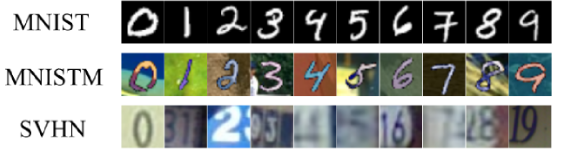
\includegraphics[width=\linewidth]{../images/domains.png}
    \caption{Ejemplos de dígitos de los tres dominios que se utilizaron}
    \label{fig:domain}
\end{figure}

Como se puede observar en la imagen~\ref{fig:domain} se trabajó con tres conjuntos de datos de dígitos (0-9) que presentan diferencias visuales importantes entre sí. MNIST es un conjunto de 70000 digitos escritos a mano en escala de grises, MNIST-M son 59.000 digitos sobre fondos fotográficos a color y SVHN presenta 99.289 dígitos en imágenes de casas reales. Los tres datasets fueron divididos en train, validation y test.

Dado que los conjuntos no comparten el mismo formato de imagen, fue necesario aplicar una etapa de preprocesamiento antes del entrenamiento. En particular, se unificó el tamaño de todas las imágenes a 32×32 píxeles y se llevó la cantidad de canales a tres. Esto implicó convertir las imágenes de MNIST, originalmente en escala de grises, a una representación RGB de tres canales, para que tuvieran la misma dimensionalidad que MNIST-M y SVHN. Además, las imágenes fueron normalizadas utilizando la media y el desvío estándar correspondientes a cada dataset. Este procedimiento permitió que todos los modelos recibieran entradas con la misma forma.

\subsection{Entrenamiento episódico y configuración few-shot}
Para entrenar los modelos de meta-learning se puede utilizar un esquema de muestreo episódico. A diferencia del entrenamiento supervisado tradicional, donde el modelo aprende a partir de batches formados aleatoriamente sobre todo el conjunto de datos, en el entrenamiento episódico cada batch simula una pequeña tarea de clasificación few-shot. De esta manera, el modelo no aprende solamente a clasificar un conjunto fijo de clases, sino a adaptarse a tareas nuevas construidas con pocos ejemplos.

Cada episodio se define mediante tres parámetros principales: $N$, $K$ y $Q$. El valor $N$ indica la cantidad de clases muestreadas en ese episodio. El valor $K$ indica la cantidad de ejemplos etiquetados disponibles por clase en el conjunto de soporte (\textit{support set}). Finalmente, $Q$ indica la cantidad de ejemplos de consulta por clase, es decir, las imágenes del \textit{query set} sobre las cuales se evalúa el desempeño del modelo dentro del episodio. Los parámetros se presentan como ``$N$-way, $K$-shot, $Q$=q".

\subsection{Prototypical Networks}
Las \textit{Prototypical Networks} (ProtoNets), propuestas por \textit{Snell et al.} (2017)\footnote{\url{https://arxiv.org/abs/1703.05175}}, son un método de meta learning diseñado para tareas de clasificación few-shot. La idea principal consiste en aprender un espacio de embeddings donde ejemplos pertenecientes a una misma clase se agrupen bien.

Durante cada episodio de entrenamiento, el modelo recibe un conjunto de soporte y un conjunto de consulta. Para cada clase $n$, se calcula un ``prototipo'' como el promedio de los embeddings de las muestras de soporte:

\begin{equation}
c_n = \frac{1}{K}
\sum_{\substack{(x,y)\in D^{\text{tr}} \\ y=n}}
f_\theta(x),
\end{equation}

donde $f_\theta(x)$ es el embedding resultante de la red $f_\theta$ para la muestra $x$, $K$ es el número de muestras de soporte por clase, y $D^{\text{tr}}$ es el conjunto de soporte.

Luego, la probabilidad de que una imagen de query $x$ pertenezca a la clase $n$ es:

\begin{equation}
p_\theta(y=n|x) =
\frac{
\exp\left(-\|\left(f_\theta(x)-c_n\right)\|^2\right)
}{
\sum_{n'} \exp\left(-\|\left(f_\theta(x)-c_{n'}\right)\|^2\right)
}.
\end{equation}

La actualización de pesos utiliza la métrica de entropía cruzada sobre esa probabilidad.

\subsection{MAML}
\textit{Model-Agnostic Meta-Learning} (MAML), propuesto por \textit{Finn et al.} (2017)\footnote{\url{https://arxiv.org/abs/1703.03400}}, es otro enfoque cuyo objetivo es aprender una inicialización de parámetros capaz de adaptarse rápidamente a nuevas tareas mediante unas pocas iteraciones de descenso por gradiente.

Durante cada episodio, el modelo realiza una adaptación interna utilizando el conjunto de soporte:

\begin{equation}
\theta'_i = \theta - \alpha \nabla_\theta
\mathcal{L}_{\mathcal{T}_i}^{support}(\theta),
\end{equation}

con $\alpha$ el learning rate y $\theta'_i$ los parámetros adaptados para la tarea $\mathcal{T}_i$.

Posteriormente en el \textit{outer loop} se evalúa el desempeño sobre el conjunto de consulta y se optimizan los parámetros originales minimizando:

\begin{equation}
\min_\theta \sum_{\mathcal{T}_i}
\mathcal{L}_{\mathcal{T}_i}^{query}(\theta'_i).
\end{equation}

Al minimizar por gradiente descendiente, se necesitan calcular gradientes de segundo orden.

A diferencia de métodos basados en métricas, MAML aprende explícitamente cómo adaptarse mediante gradientes, permitiendo una rápida especialización a nuevas tareas. Sin embargo, el entrenamiento puede resultar inestable y computacionalmente costoso debido al cálculo de gradientes de segundo orden.

\subsection{ProtoMAML}

ProtoMAML, propuesto por \textit{Triantafillou et al.} (2020)\footnote{\url{https://arxiv.org/abs/1903.03096}}, combina ideas de Prototypical Networks y MAML. El objetivo es aprovechar la estabilidad de los métodos métricos junto con la capacidad de adaptación rápida basada en optimización.

En ProtoMAML, los prototipos calculados a partir del conjunto de soporte se utilizan para inicializar dinámicamente la capa clasificadora antes de realizar las actualizaciones internas de MAML. Dados los prototipos $\mathbf{p}_c$, los pesos y sesgos del clasificador se inicializan como:

\begin{equation}
w_c = 2p^{\intercal}_c,
\end{equation}

\begin{equation}
b_c = -\|p_c\|^2.
\end{equation}

Este método, en teoría, produce predicciones equivalentes a las Prototypical Networks. Luego, a partir de este punto de partida, los pasos de adaptación refinan los parámetros logrando converger en considerablemente menos pasos que una inicialización aleatoria.

\subsection{DANN}

La \textit{Domain-Adversarial Neural Network} (DANN), propuesta por \textit{Ganin et al.} (2016)\footnote{\url{https://arxiv.org/abs/1505.07818}}, es un método de domain adaptation cuyo objetivo es aprender representaciones invariantes al dominio.

La arquitectura consta de tres componentes principales: un extractor de características, un clasificador de etiquetas y un clasificador de dominio.

El extractor de características se entrena para minimizar simultáneamente el error de clasificación y maximizar el error del clasificador de dominio. Esto se logra mediante una capa denominada \textit{Gradient Reversal Layer} (GRL), que invierte el signo del gradiente durante la retropropagación.

La función objetivo puede expresarse como:

\begin{equation}
\mathcal{L}_{DANN} =
\mathcal{L}_{task} - \lambda \mathcal{L}_{domain},
\end{equation}

donde $\mathcal{L}_{task}$ corresponde a la pérdida de clasificación principal y $\mathcal{L}_{domain}$ a la pérdida del discriminador de dominio. El valor de $\lambda$ aumenta a lo largo del entrenamiento para que el encoder pueda construir buenos features iniciales con menor intervención de $\mathcal{L}_{domain}$.

\begin{equation}
    \lambda_p = \frac{2}{1 + e^{-10p}} - 1, \qquad p \in [0, 1]
\end{equation}

De esta manera, el modelo aprende a clasificar y a confundir al discriminador simultáneamente, generando embeddings útiles pero indistinguibles entre dominios fuente y objetivo. Esto favorece la generalización ante un \textit{domain shift}.   

\section{Desarrollo}
Por recomendación de la cátedra, el encoder compartido entre todos los modelos testeados parte de una arquitectura ConvNet de 4 bloques. El único detalle es un cambio de normalización por bache a por grupos, dado que se encuentra mejor rendimiento de MAML y ProtoMAML con bache de tamaño 1, y la normalización por grupos es más efectiva en baches pequeños. En todos los experimentos, el encoder recibió imágenes de tres canales, utilizó una dimensión oculta y de embedding de 64.

Los métodos de meta-learning se entrenaron solamente sobre MNIST. Se incluyen MNIST-M y SVHN para reportar accuracy de support y validation, así como las proyecciones de t-SNE de los embeddings del modelo resultante. MAML también incluye análisis adicionales relacionados al efecto del inner y outer loop sobre la accuracy.

En cuanto a los hiperparámetros, los valores de $N$, $K$ y $Q$ siguieron la configuración definida por la cátedra. Todos los modelos episódicos trabajan con una configuración 5-way y $Q=15$, mientras que el valor de $K$ varía según el modelo: ProtoNet fue entrenado en 5-shot, mientras que MAML y ProtoMAML en 1-shot.

En el caso de ProtoNet, el modelo fue entrenado durante 200 épocas de 100 episodios cada una, con un \textit{learning rate} de $0.001$. En cambio, MAML y ProtoMAML fueron entrenados con un tamaño de meta bache de 1, durante 10.000 meta-iteraciones.

MAML realizó dos actualizaciones internas antes de la actualización externa, con un learning rate interno de $0.009$ y uno externo de $0.0009$. Por su parte, ProtoMAML realizó una única actualización interna antes de la actualización externa, con un learning rate interno de $0.01$ y uno externo de $0.001$.

Además, para analizar el efecto de la cantidad de ejemplos disponibles por clase, se evaluó el desempeño de los modelos variando $K$ en los valores $1, 2, 4, 8$ y $16$, para 1000 episodios sobre el set de testeo.

Para domain adaptation, se entrenan tres versiones de DANN: una estándar, una sin discriminador para usar como \textit{baseline} y un baseline \textit{finetuned}. MNIST-M se incluye durante el entrenamiento para GRL en DANN normal y para \textit{finetuning} del baseline.

Ambos baselines sirven como referencia para medir el rendimiento de DANN: el baseline normal es el \textit{lower bound}, donde solo se puede entrenar con los datos de MNIST; el baseline finetuned es el \textit{upper bound}, que usa las etiquetas del dominio objetivo para ajustar. En comparación, DANN es un punto medio ya que usa datos no etiquetados del dominio objetivo, un caso más realista donde la recolección es fácil pero el etiquetado es costoso.

Los tres entrenamientos se realizaron con un tamaño de bache de 512 y un learning rate de $0.001$. El baseline fue entrenado durante 150 épocas, luego se aplicó fine-tuning durante 150 épocas adicionales, mientras que el DANN estándar fue entrenado durante 300 épocas.

\end{multicols}
% \newpage
\section{Resultados}
\subsection{Prototypical Networks}
\begin{table}[h!]
\centering

\begin{tabular}{|l|c|c|}
\hline
 & Support (\%) & Query (\%)\\
\hline
Train & 99.96 & 99.84\\
\hline
Validation & 99.72 & 99.39\\
\hline
\end{tabular}
\caption{Accuracies finales de ProtoNet sobre MNIST para support y query.}
\label{tab:proto accs}
\end{table}

En la tabla~\ref{tab:proto accs} se registran las accuracies conseguidas por ProtoNet. El alto rendimiento del support set se explica, en su mayor parte, por el hecho de que es el mismo conjunto sobre el que se calculan los prototipos. El resultado principal de la tabla es la accuracy casi igual conseguida por query, indicando que los prototipos construidos a partir de support logran generalizar correctamente a ejemplos no vistos dentro de cada tarea.

\begin{figure}[H]
    \centering
    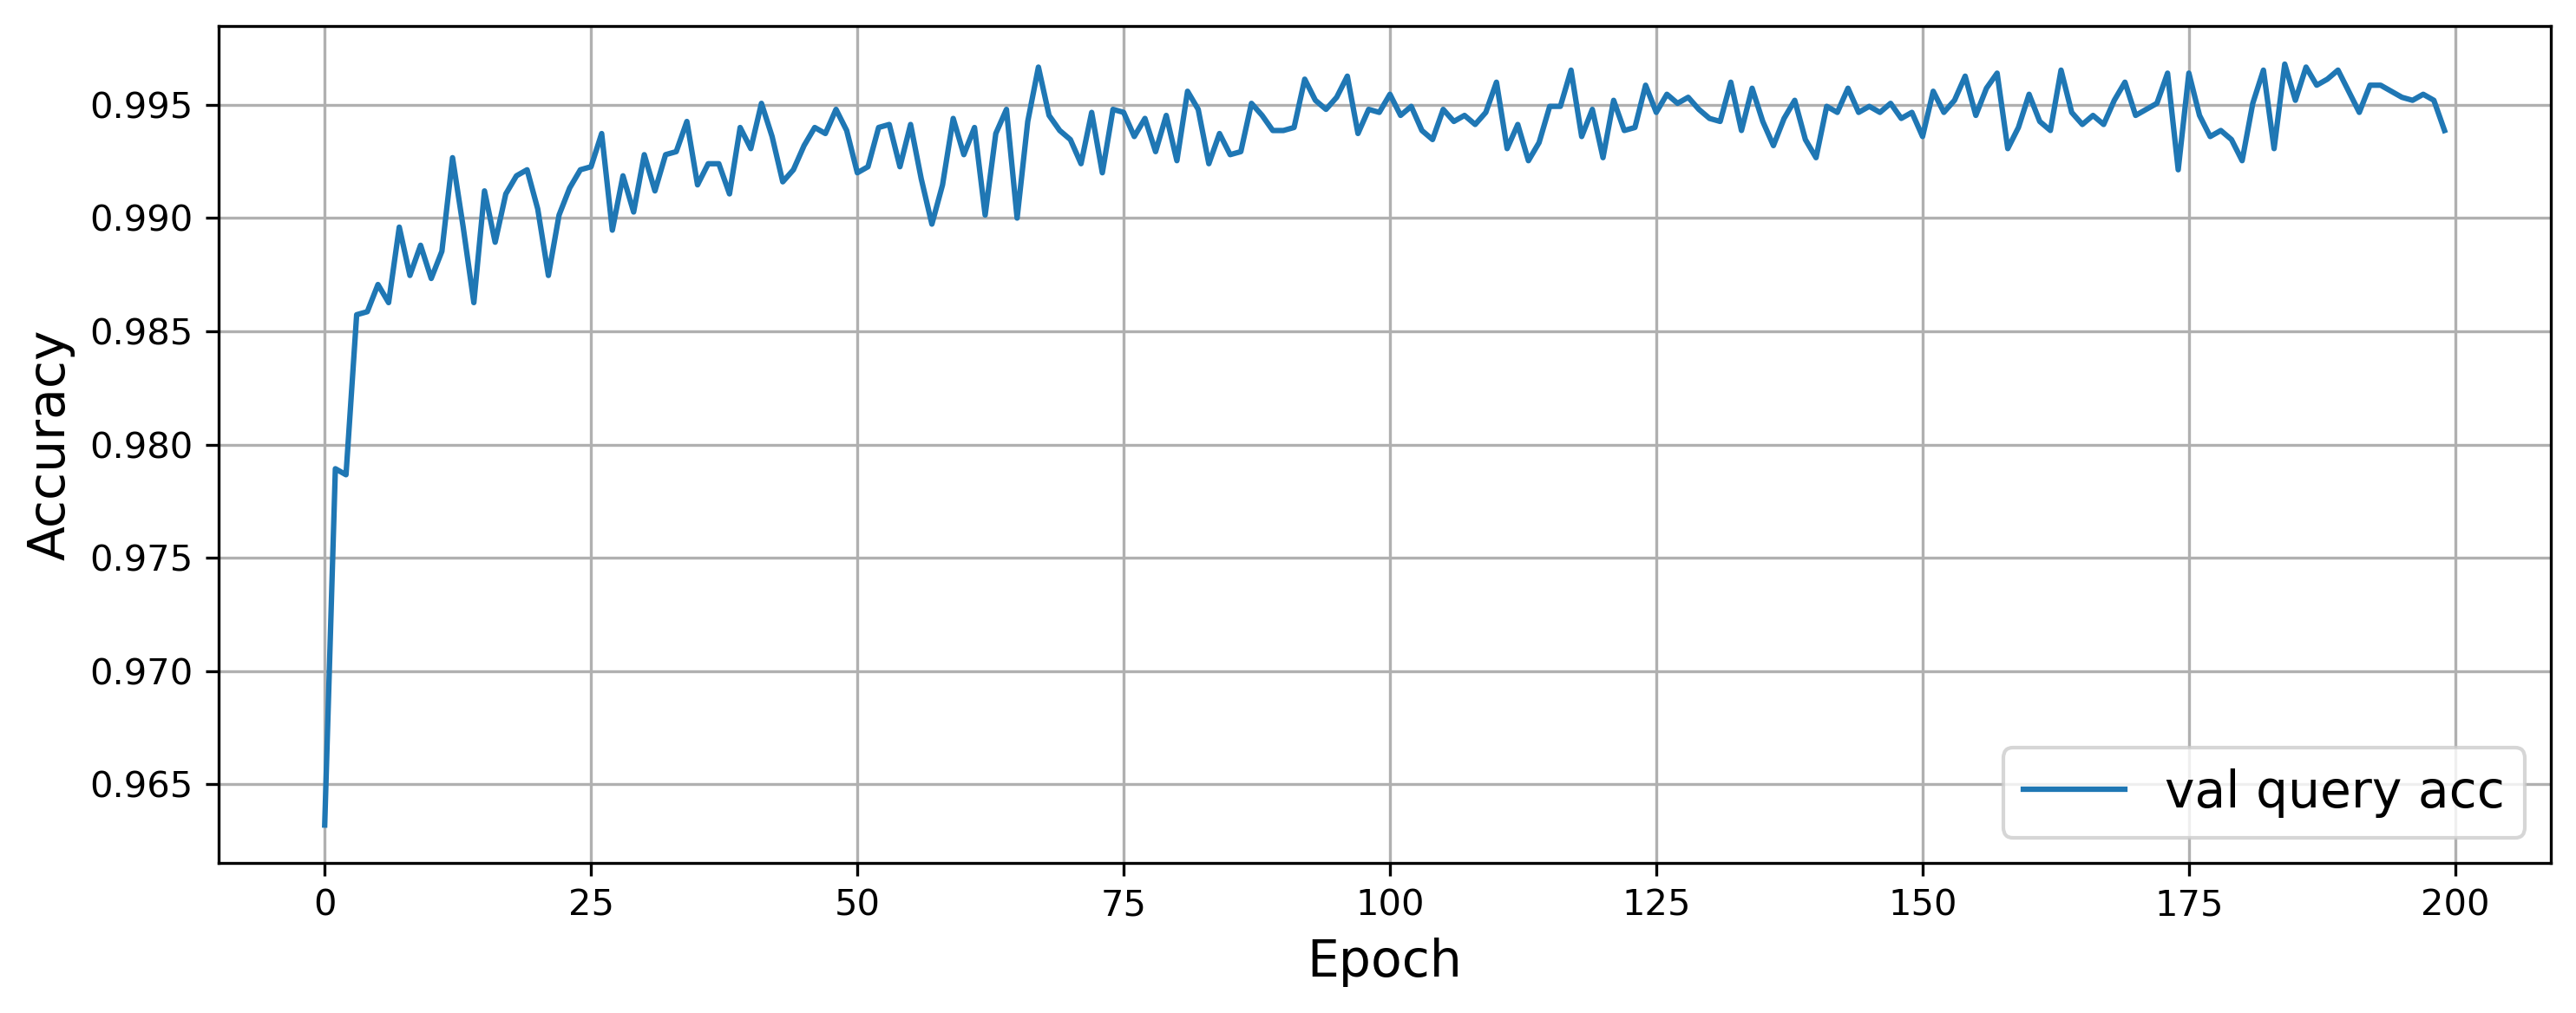
\includegraphics[width=0.8\textwidth]{../images/protonet/protonet_training.png}
    \caption{Accuracy de query en validación a lo largo del entrenamiento. }
    \label{fig:protonet training}
\end{figure}

% ¿Se forman clusters separados? ¿Cómo evoluciona la estructura a medida que avanza el entrenamiento?

En la figura~\ref{fig:protonet training} se muestra la evolución de la accuracy sobre el set de validación de query. Se observa un incremento rápido durante las primeras épocas y luego una oscilación en valores altos cercanos a 0.995. Esa oscilación surge del sampleo realizado durante el entrenamiento. 

\begin{figure}[H]
    \centering
    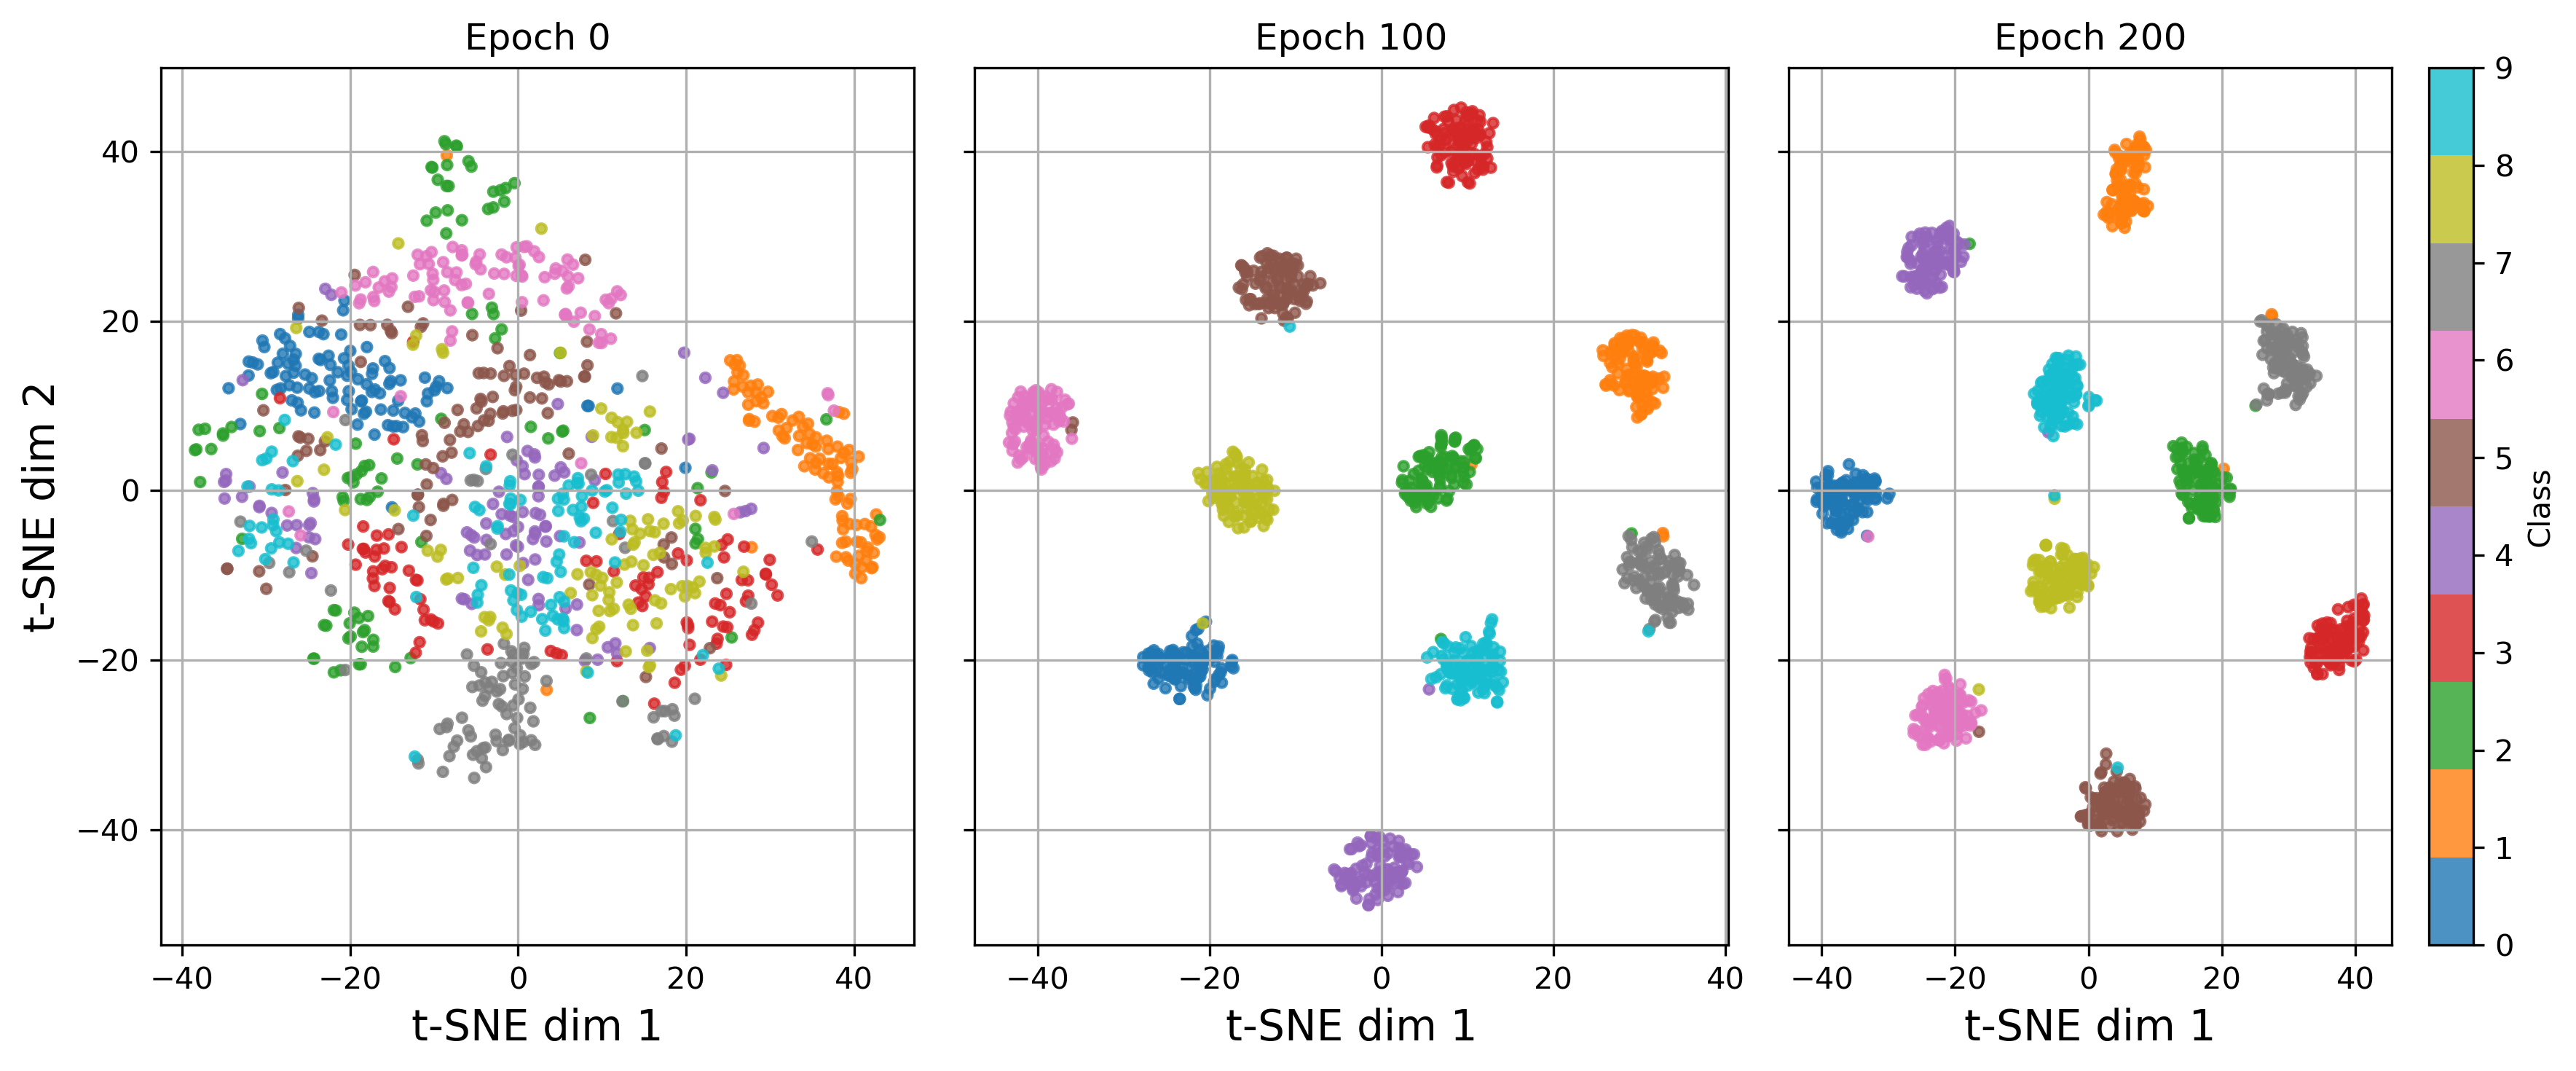
\includegraphics[width=0.8\textwidth]{../images/protonet/protonet_training_tsnes.png}
    \caption{t-SNE de los embeddings del encoder para un conjunto de imágenes de MNIST al inicio, a mitad y al final del entrenamiento.}
    \label{fig:protonet training tsnes}
\end{figure}

% ¿Se forman clusters separados? ¿Cómo evoluciona la estructura a medida que avanza el entrenamiento?

En la figura~\ref{fig:protonent training tsnes} se visualiza la evolución de los embeddings generados por el encoder sobre un conjunto de imágenes de MNIST. Antes del entrenamiento, las clases estan mayormente mezcladas y solo la clase 1 parece formar una especie de cluster con pocas muestras dispersas. En la época 100, en cambio, ya se distinguen clusters separados por clases, con pocas muestras mal distribuidas. Finalmente para la época 200 no se produce un cambio significativo.

\begin{figure}[H]
    \centering
    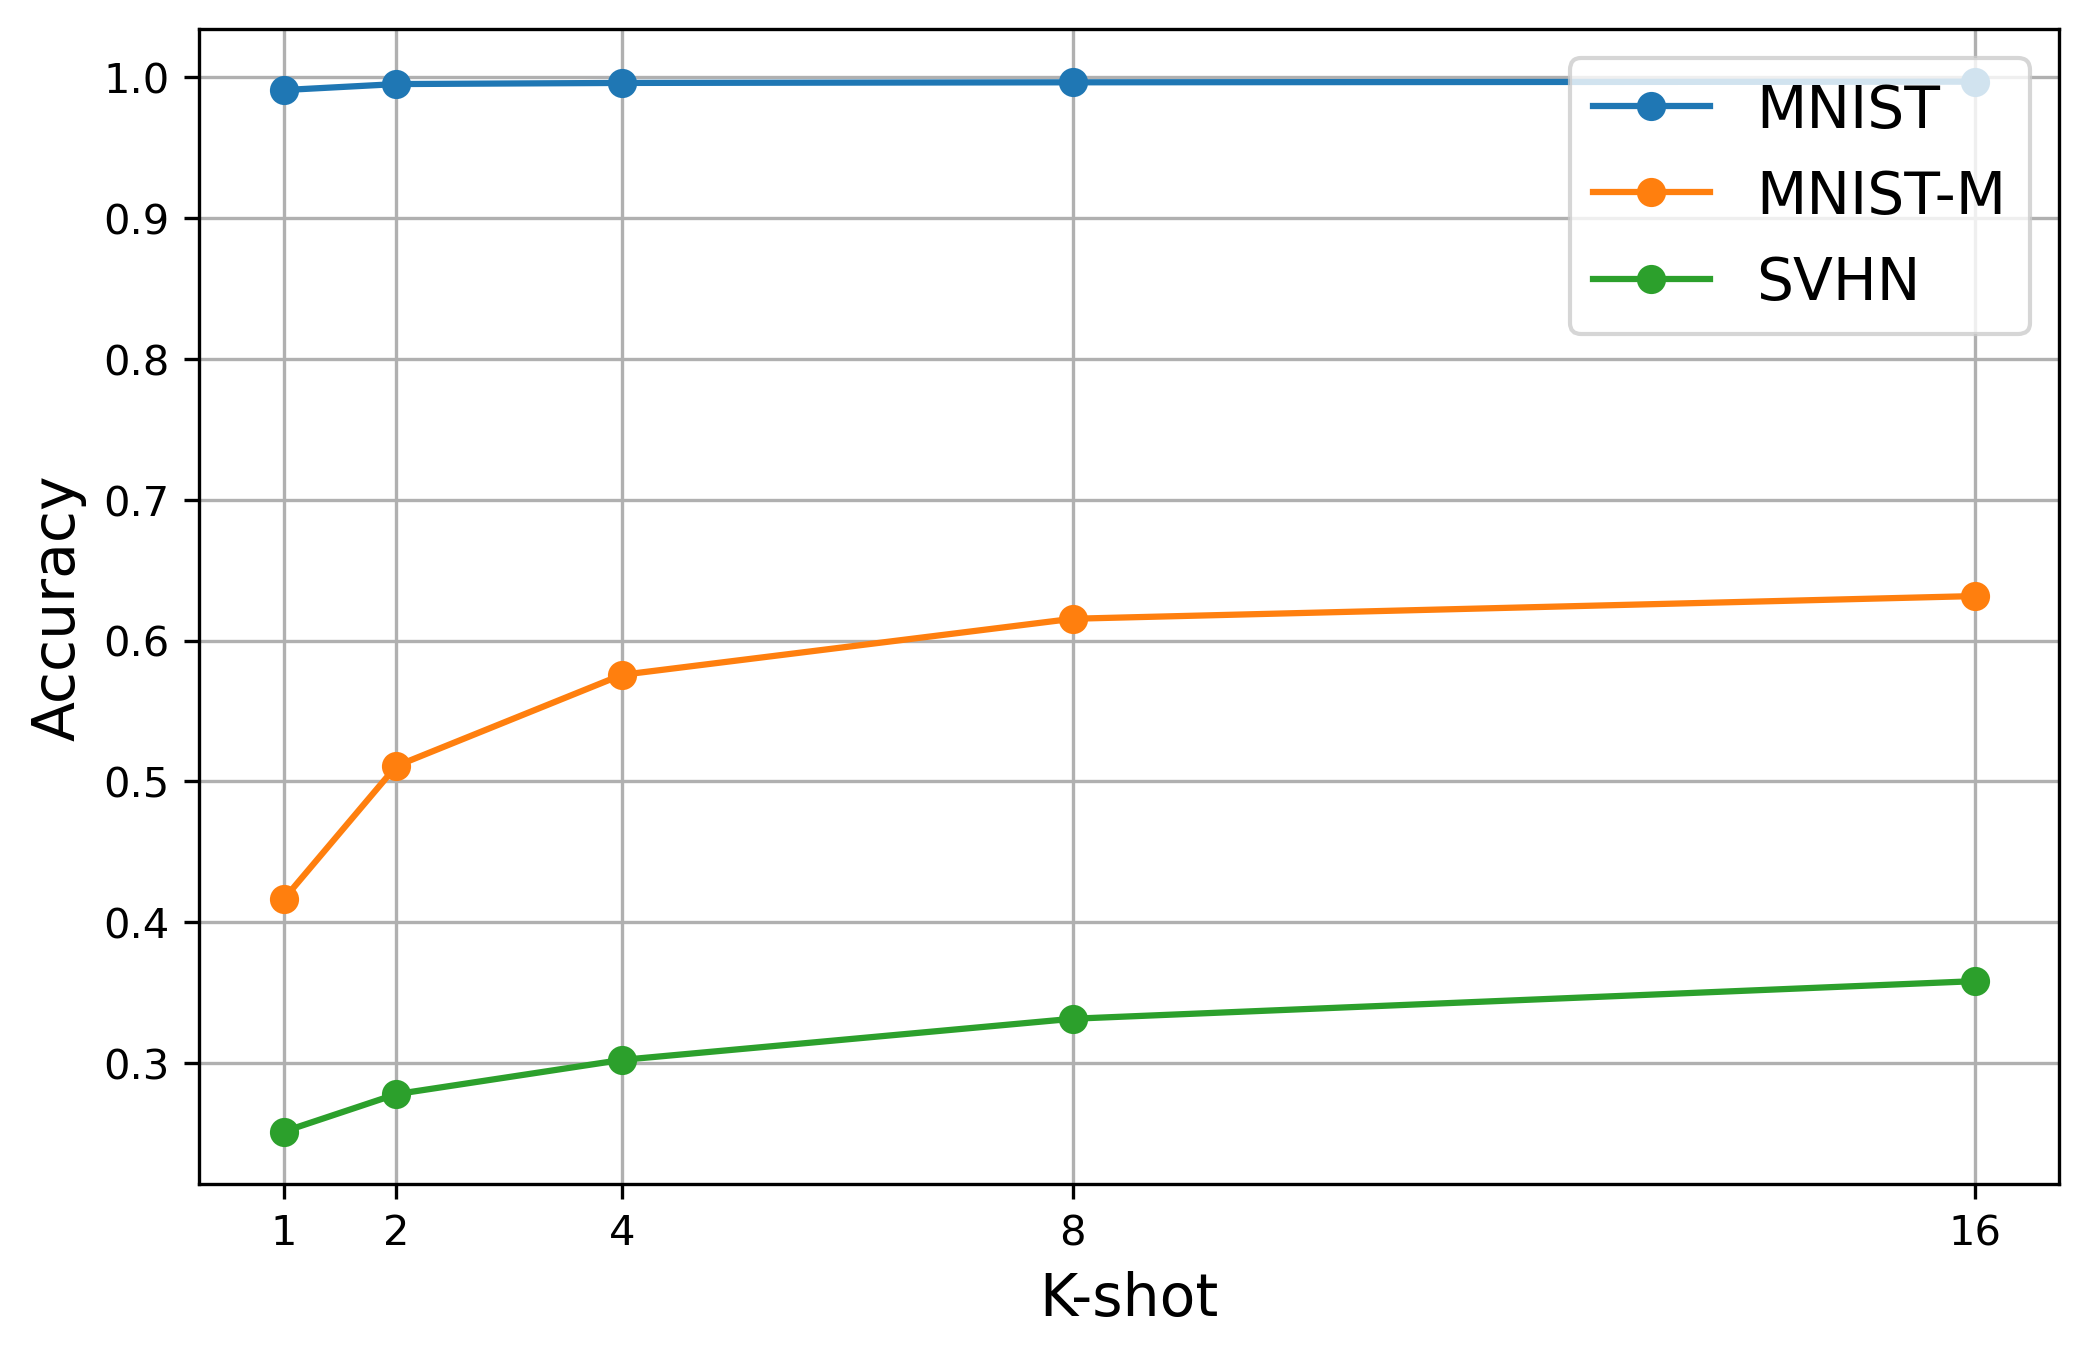
\includegraphics[width=0.6\textwidth]{../images/protonet/acc_vs_ks.png}
    \caption{Accuracy sobre el conjunto de test de MNIST con k = {1, 2, 4, 8, 16}.}
    \label{fig:protonet acc vs k}
\end{figure}

En la imagen~\ref{fig:protonet acc vs k} se evaluó el modelo sobre los conjuntos de testeo de todos los dominios para distintas $K$. 

En MNIST se observa una accuracy casi perfecta para todo $K$, dado que el modelo entrenó sobre esos datos y las figuras~\ref{fig:protonet training} y~\ref{fig:protonent training tsnes} demuestran que logra diferenciar y generalizar correctamente entre clases. Aumentar el valor de $K$ casi no modifica el desempeño ya que con una baja cantidad de ejemplos, los prototipos ya resultan lo suficientemente representativos.

En cambio, para los dominios MNIST-M y SVHN, la accuracy es considerablemente menor pero siempre creciente junto a $K$. También puede notarse que MNIST-M mantiene una accuracy de aproximadamente el doble de valor que SVHN para todos los valores de $K$. Esto puede explicarse por la similaridad entre MNIST y MNIST-M al ser el ultimo una modificación del primero, mientras que SVHN presenta un desplazamiento de dominio más fuerte.

También se considera necesario remarcar la forma de crecimiento de la accuracy junto a $K$. EN MNIST-M y SVHN, el aporte de cada muestra a la generación de prototipos es menor, indicando que no es necesario incluir todo el dataset para generar prototipos representativos.

\begin{figure}[H]
    \centering
    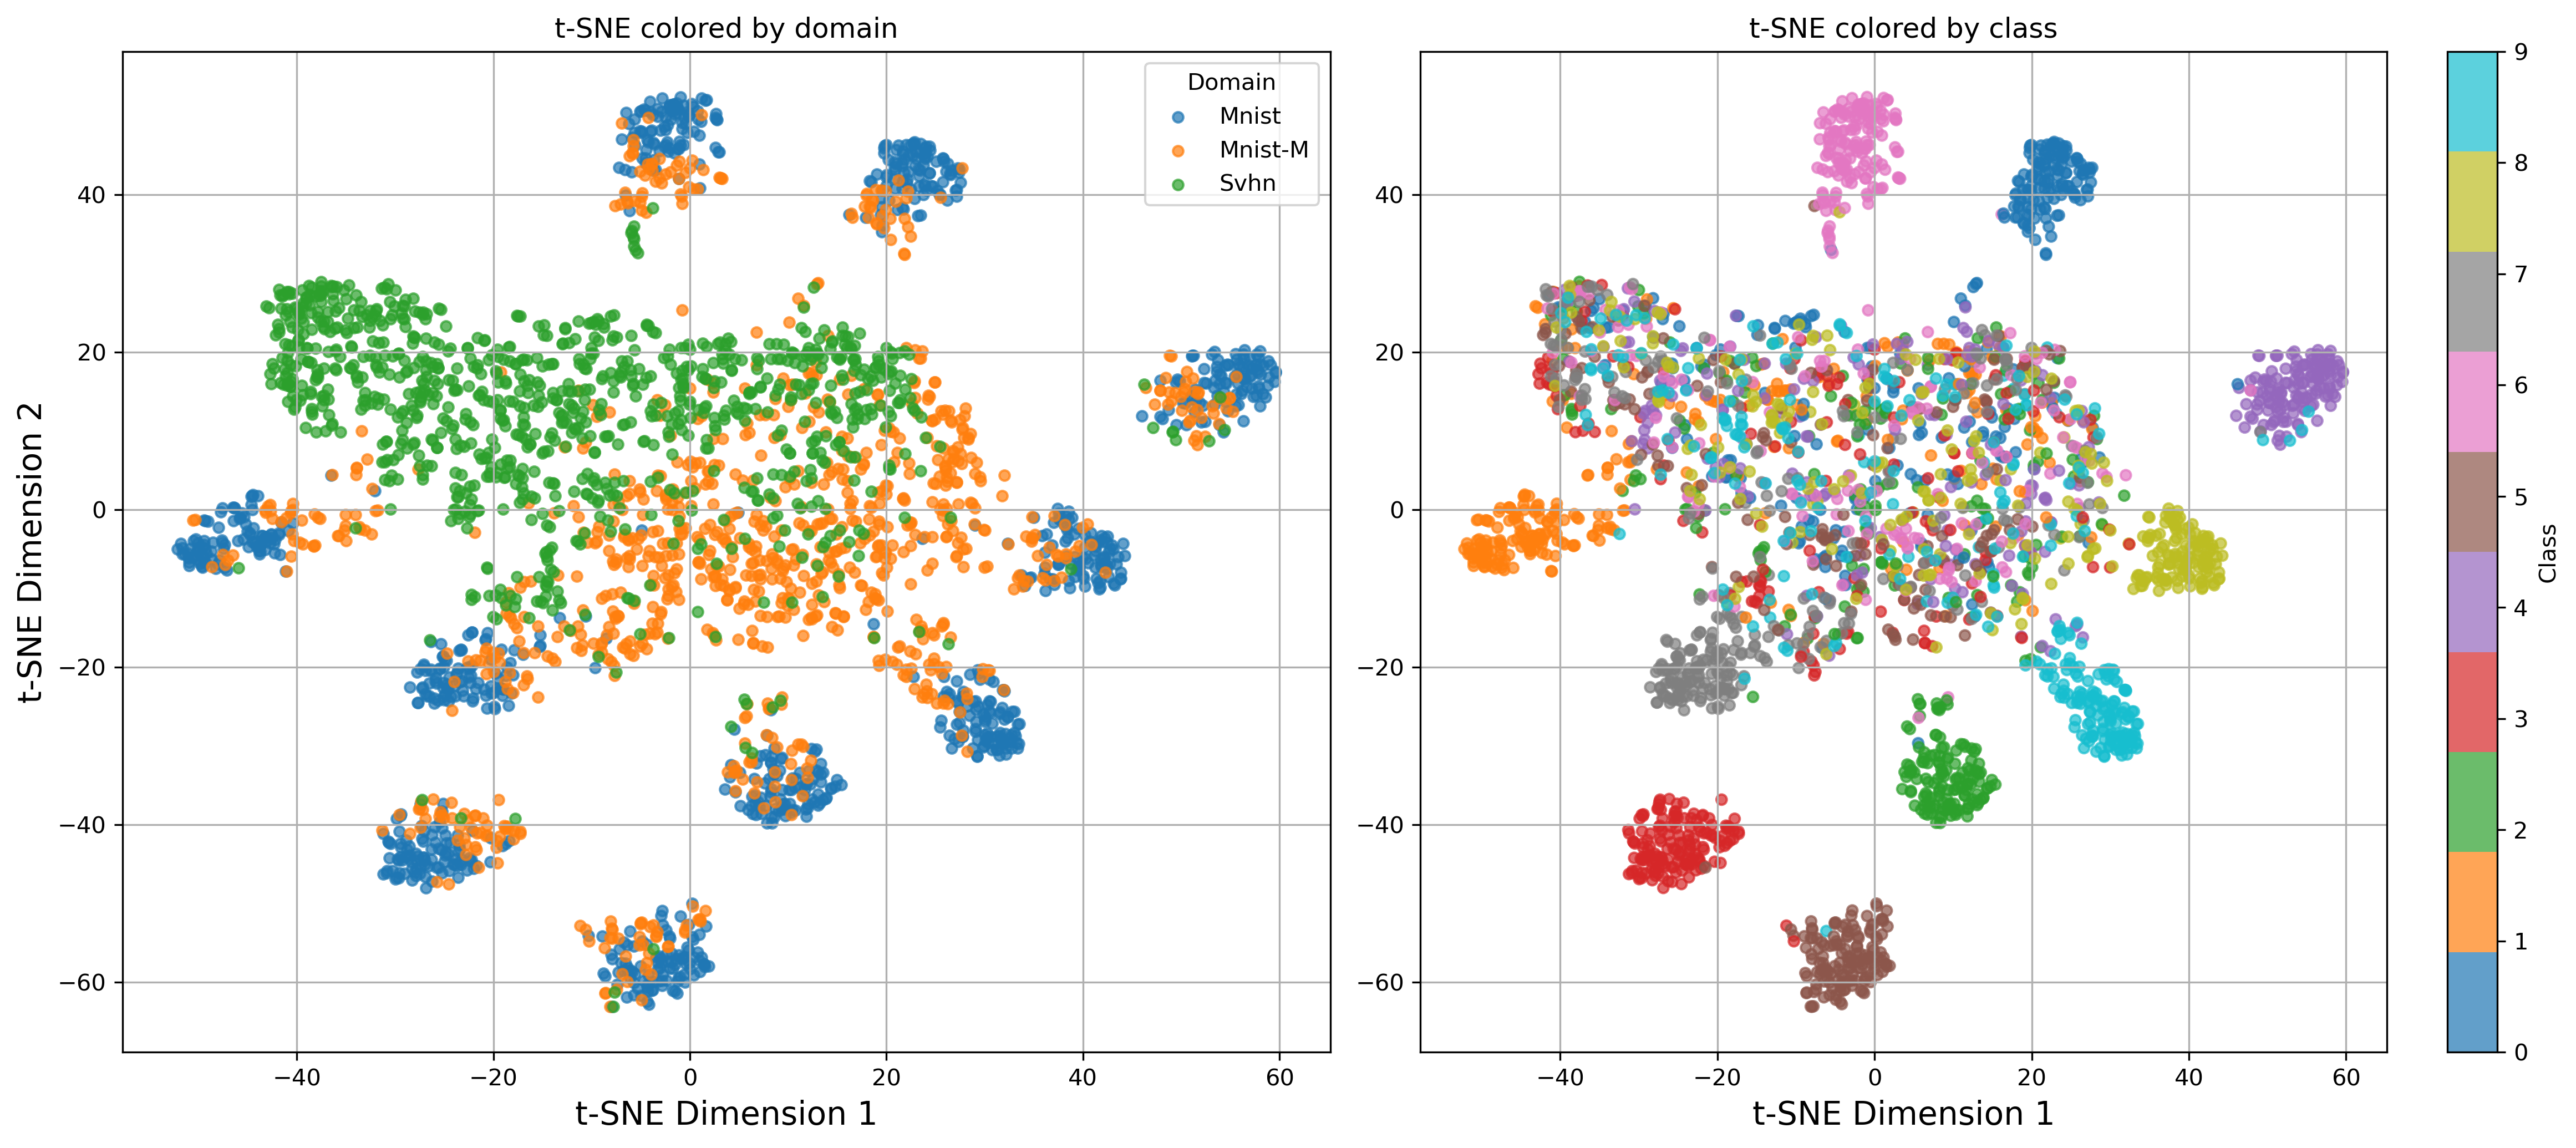
\includegraphics[width=0.8\textwidth]{../images/protonet/tsnes_domain_class.png}
    \caption{t-SNE de los embeddings del encoder para un conjunto de imágenes de prueba sobre los tres dominios.}
    \label{fig:protonet tsnes}
\end{figure}

% ¿Están los embeddings de los mismos dígitos cerca entre dominios? ¿Qué implica esto para la clasificación episódica cross-domain

En la figura~\ref{fig:protonet tsnes} se visualizan los embeddings producidos por el encoder, coloreados tanto por dominio como por clase. En el gráfico por dominio se observa que MNIST tiende a formar grupos más compactos y separados, mientras que MNIST-M aparece parcialmente superpuesto con MNIST en algunas regiones. En cambio, SVHN aparece mucho más disperso y desplazado, lo que indica una mayor diferencia de dominio.

% TEO: otra versión
%Al comparar con el gráfico coloreado por clase, se nota que los clusters definidos corresponden correctamente a distintos dígitos, con un pequeño error para muestras de MNIST-M y SVHN. Sin embargo, la zona central dispersa, con mezcla entre clases, indica que los embeddings de un mismo dígito no se clusterizan correctamente a través de dominios. Esto implica que, en clasificación episódica cross-domain, los prototipos construidos a partir del support set pueden dejar de ser representativos para clasificar correctamente las muestras de query cuando el dominio cambia demasiado.

Al observar el gráfico coloreado por clase, se ve que algunos dígitos forman clusters definidos, pero también existe una zona central con mucha mezcla entre clases, indicando que los embeddings de un mismo dígito no pudieron quedar cerca entre dominios. En particular, algunas muestras de MNIST-M parecen alinearse con las de MNIST, mientras que las de SVHN se integran mucho menos en los clusters aprendidos. Esto implica que, en clasificación episódica cross-domain, los prototipos construidos a partir del support set pueden dejar de ser representativos para clasificar correctamente las muestras de query cuando el dominio cambia demasiado.


\subsection{MAML}


\begin{figure}[H]
    \centering
    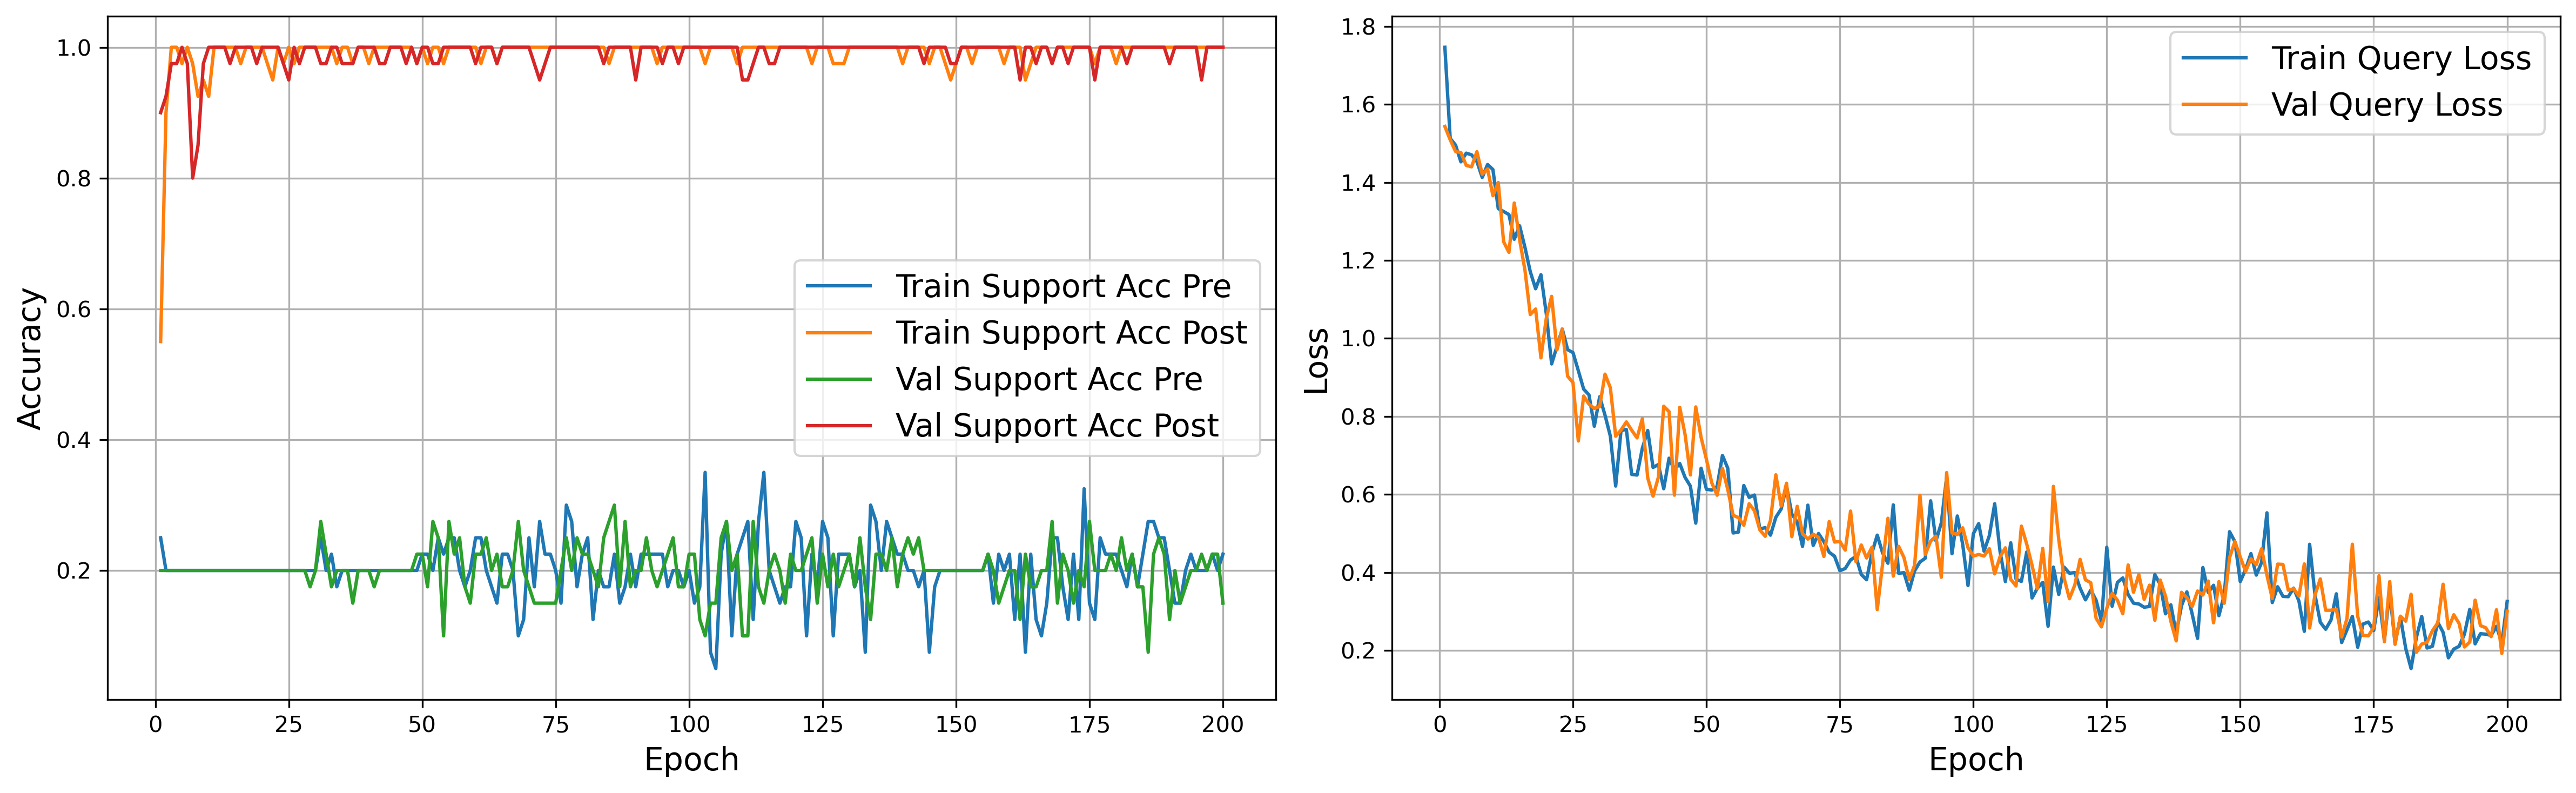
\includegraphics[width=0.8\textwidth]{../images/maml/maml_training.png}
    \caption{Accuracy post adaptación en validación durante el entrenamiento}
    \label{fig:maml training}
\end{figure}

\begin{table}[h!]
\centering

\begin{tabular}{|l|c|c|c|}
\hline
 & Support pre (\%) & Support post (\%) & Query post(\%)\\
\hline
Train & 20 & 100 & 93.33\\
\hline
Validation & 20 & 100 & 92\\
\hline
\end{tabular}
\caption{Accuracies finales de MAML sobre MNIST para support (pre y post) y query (post).}
\label{tab:maml accs}
\end{table}

En la figura~\ref{fig:maml training} se observa la evolución de la accuracy sobre el support set de validación luego de la adaptación interna de MAML. La curva presenta un comportamiento ruidoso, esperable en un entrenamiento episódico con tamaño de meta bache 1. A pesar de estas oscilaciones, la accuracy se mantiene mayormente en valores altos, entre 0.8 y 1.0, lo que indica que el modelo logra ajustarse correctamente a los ejemplos del support set después de los pasos internos de adaptación. Dado que se trabaja en un esquema 5-way 1-shot, el support set contiene solo cinco ejemplos, por lo que la métrica toma valores discretos y puede presentar saltos bruscos entre iteraciones.

La tabla~\ref{tab:maml accs} confirma este comportamiento: antes de la adaptación, la accuracy sobre support es 20$\%$, equivalente al azar en una tarea de cinco clases. Después de la adaptación, la accuracy sobre support alcanza 100$\%$, lo que muestra que el modelo consigue ajustarse perfectamente a los ejemplos disponibles en cada episodio. Sin embargo, la accuracy sobre query después de la adaptación alcanza un valor de 93.33$\%$ en entrenamiento y 92$\%$ en validación, lo que sugiere que el modelo aprende a adaptarse rápidamente a nuevas tareas y generalizar a muestras no vistas.


\subsection{Prototypical Networks, MAML y ProtoMAML}
\begin{figure}[H]
    \centering
    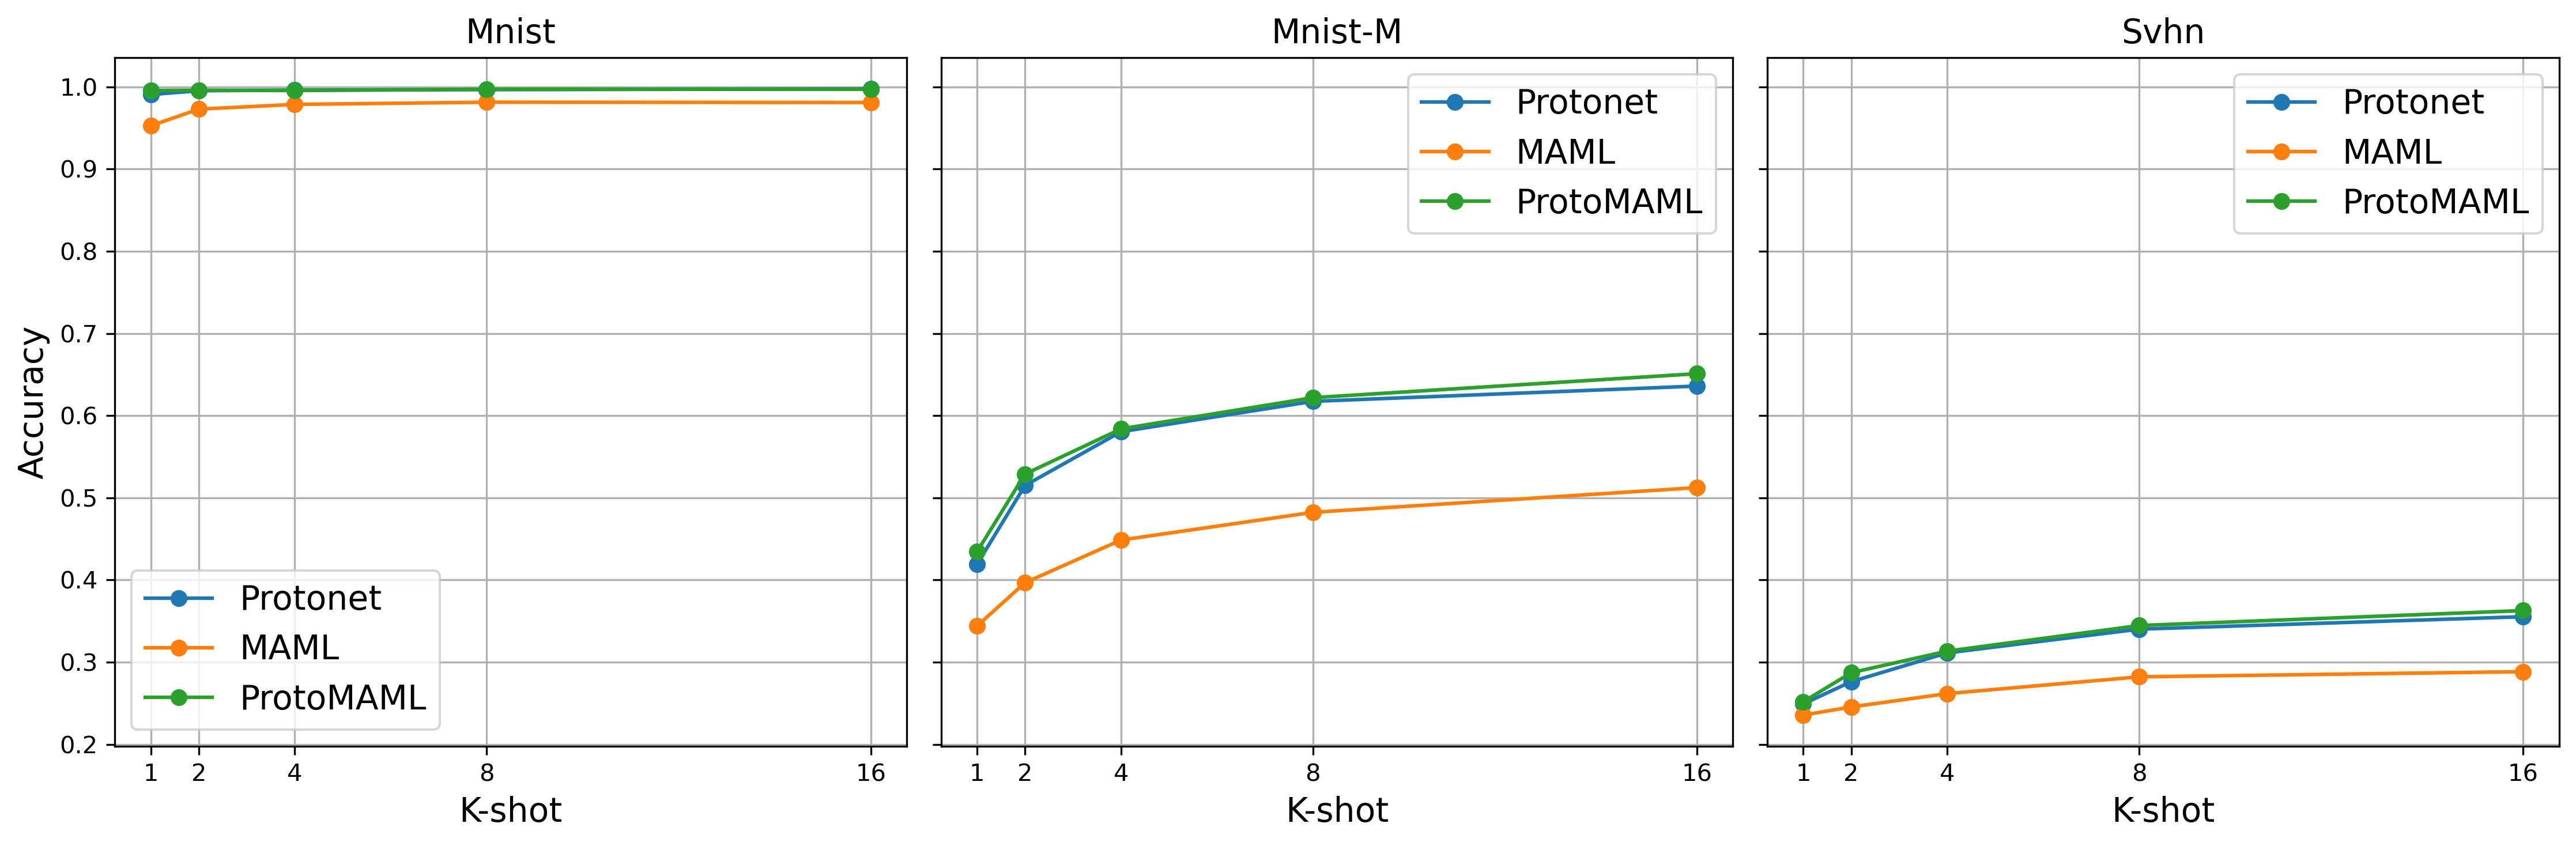
\includegraphics[width=0.9\textwidth]{../images/compare_models/accuracies_ks.png}
    \caption{Accuracy para los tres modelos sobre el conjunto de test de MNIST con k = {1, 2, 4, 8, 16}}
    \label{fig:accuracies ks models}
\end{figure}

En la figura~\ref{fig:accuracies ks models} se comparan ProtoNet, MAML y ProtoMAML para distintos valores de $K$ sobre MNIST, MNIST-M y SVHN. En MNIST, los tres modelos alcanzan accuracies cercanas a 1, lo cual era esperable por tratarse del dominio de entrenamiento. ProtoNet y ProtoMAML se mantienen levemente por encima de MAML.

En los dominios cross-domain, MNIST-M y SVHN, la diferencia entre métodos es más clara. ProtoNet y ProtoMAML obtienen mejores resultados que MAML para todos los valores de $K$, lo que sugiere que los enfoques basados en prototipos son más robustos frente al cambio de dominio.

El resultado destacado de esta figura es que ProtoMAML logra resultados similares o incluso levemente superiores a ProtoNet, aún siendo entrenado con la mitad de iteraciones (10.000 a 20.000) y un menor valor de $K$ (1 a 5). Esto parece indicar que ProtoMAML aprovecha la combinación entre representación prototípica y adaptación interna. MAML, por su parte, queda por debajo, lo que muestra que la adaptación por gradiente con pocos ejemplos no es suficiente para compensar el cambio de dominio.  

\begin{figure}[H]
    \centering
    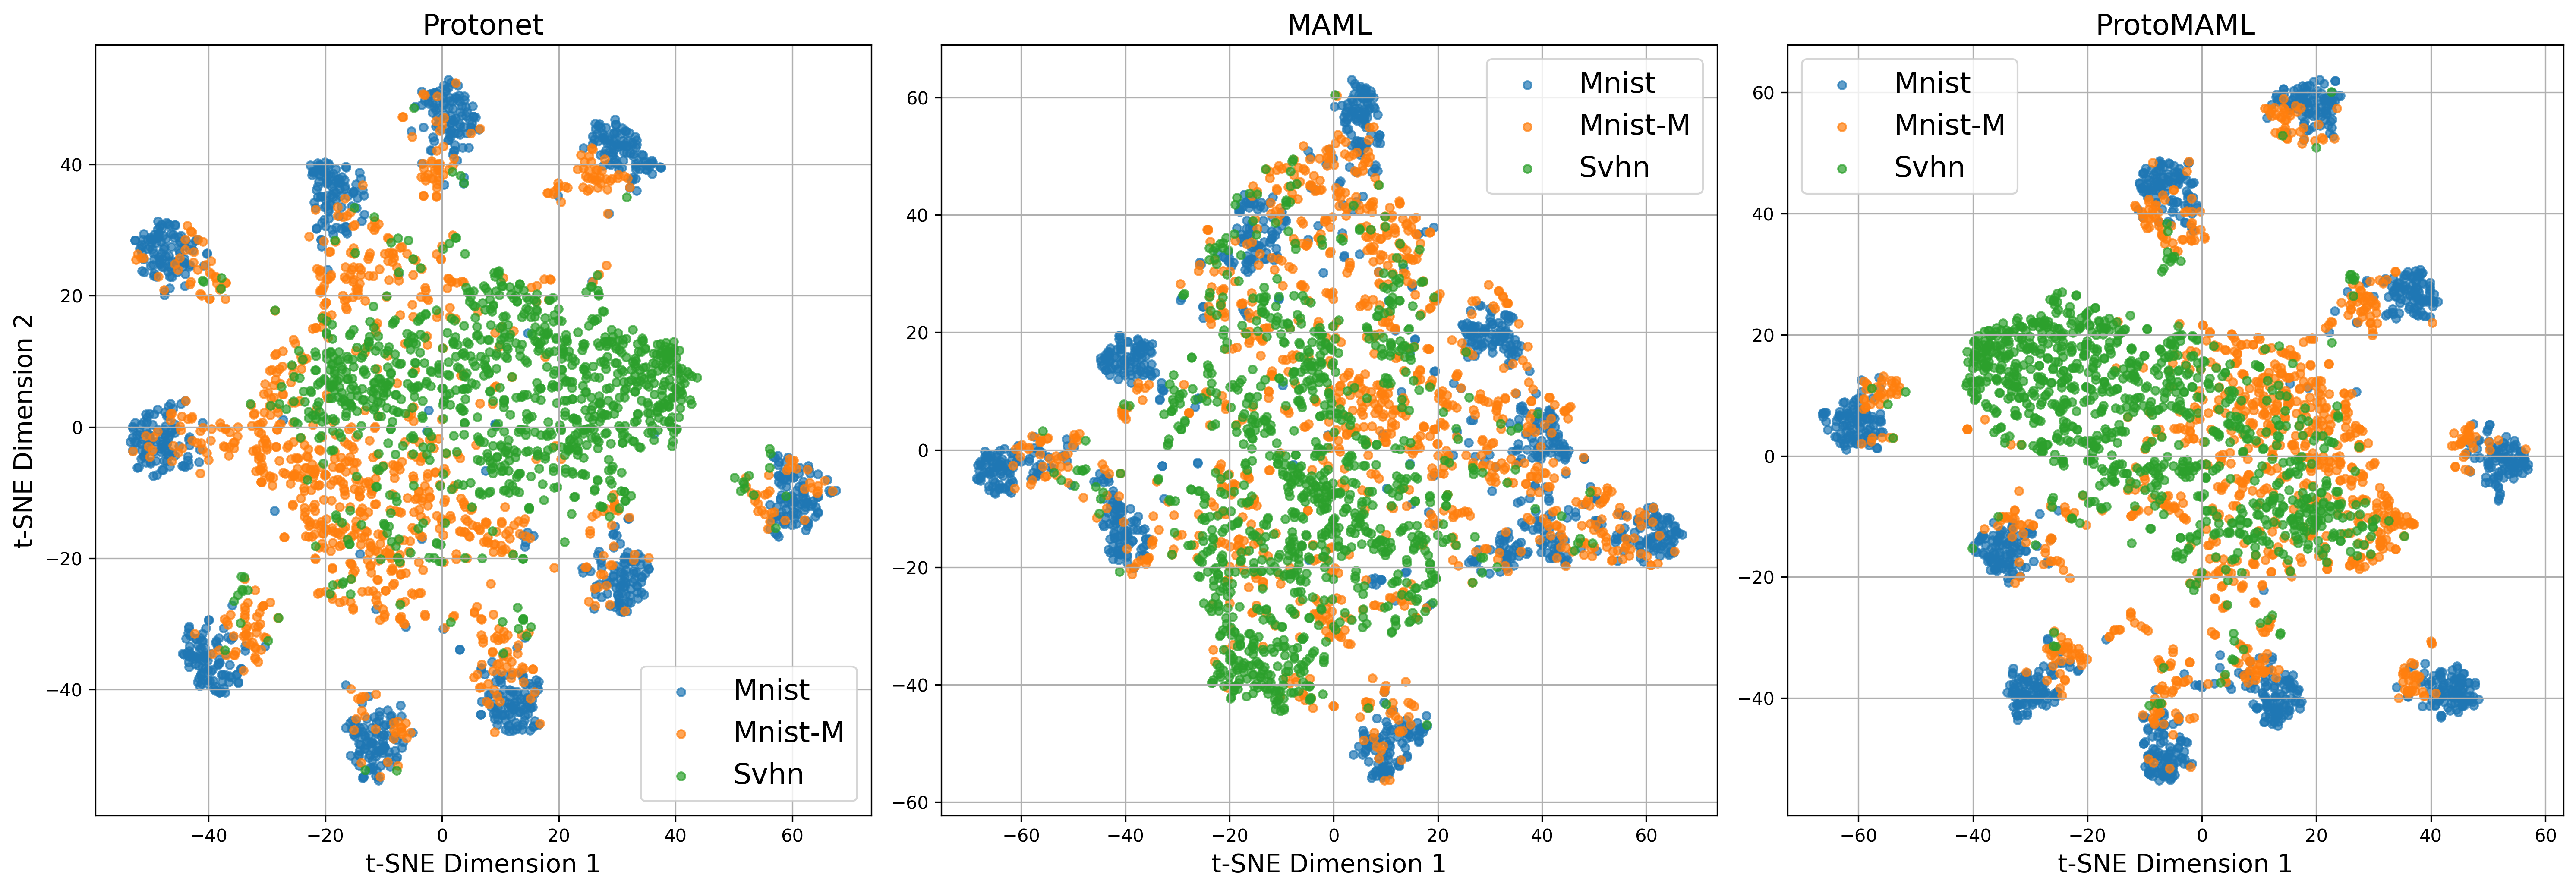
\includegraphics[width=0.8\textwidth]{../images/compare_models/models_tsnes.png}
    \caption{t-SNE de los embeddings de los encoders de los tres modelos para un conjunto de imágene de prueba sobre los tres dominios.}
    \label{fig:models tsnes}
\end{figure}


% Visualización del espacio latente comparativa: proyectar los embeddings del encoder para imágenes de MNIST, MNIST-M y SVHN en el mismo gráfico, usando el encoder de cada modelo. Colorear por dominio. ¿Qué modelo produce embeddings más cercanos entre dominios? ¿Se corresponde con la accuracy cross-domain?

En la figura~\ref{fig:models tsnes} se comparan los embeddings generados por ProtoNet, MAML y ProtoMAML, coloreados según el dominio. Se puede observar que los modelos de Protonet y ProtoMAML muestran una mayor cercanía entre los embeddings de MNIST y MNIST-M, especialmente en algunos grupos de clases donde ambos dominios aparecen parcialmente superpuestos. SVHN, en cambio, permanece más separado y disperso, lo cual coincide con sus menores valores de accuracy. MAML presenta una estructura menos alineada entre dominios, lo que se refleja también en su peor desempeño en cross-domain.


En conjunto, ProtoMAML parece producir los embeddings más cercanos entre dominios, seguido de ProtoNet. Esta observación es consistente con los resultados de accuracy mostrados en la figura~\ref{fig:accuracies ks models}, ya que ambos modelos superan a MAML en MNIST-M y SVHN.

\subsection{DANN}

\begin{figure}[H]
    \centering
    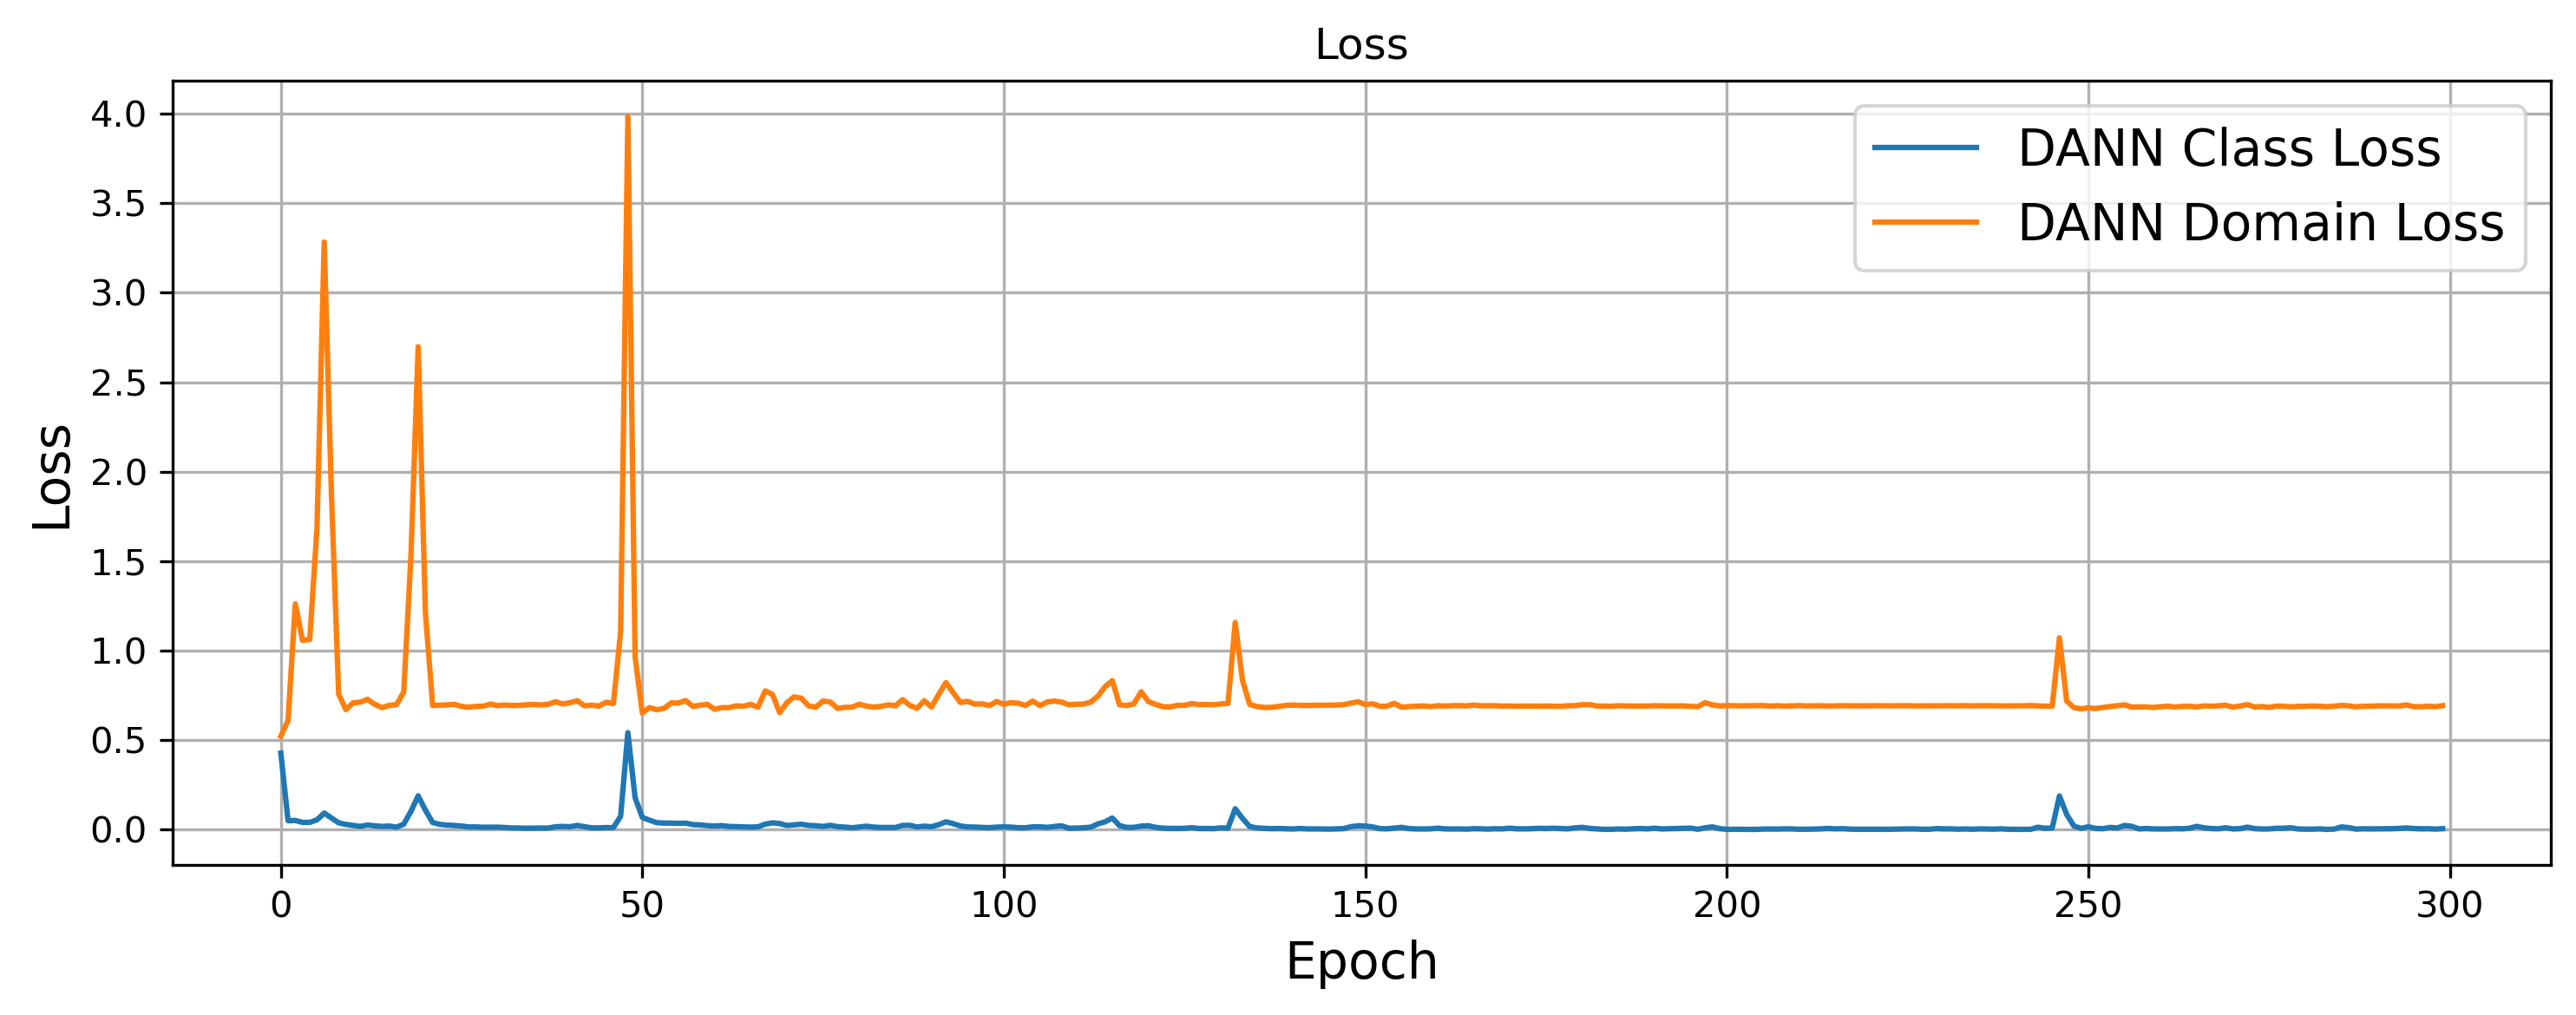
\includegraphics[width=0.8\textwidth]{../images/dann/dann_training_loss.png}
    \caption{Perdida de clasificación y dominio durante el entrenamiento de DANN.}
    \label{fig:dann loss}
\end{figure}

% Graficar en el mismo plot la loss de clasificación, la loss de dominio y la accuracy en MNIST-M a lo largo del entrenamiento, para DANN y el baseline. ¿Cómo evolucionan en relación la una con la otra?

En la figura~\ref{fig:dann loss} se tienen las pérdidas de clasificación y de dominio del modelo DANN durante el entrenamiento. Se observa que ambas tienen oscilaciones correspondientes al tipo de entrenamiento adversarial, presentando picos en epocas similares, pero perdida de dominio los presenta con escalas mayores.

Para comparar el entrenamiento del modelo DANN con el modelo baseline, en la siguiente figura se representa únicamente la pérdida de clasificación. Se omite la pérdida de dominio para facilitar la visualización, ya que su escala es considerablemente mayor y dificulta la comparación.

\begin{figure}[H]
    \centering
    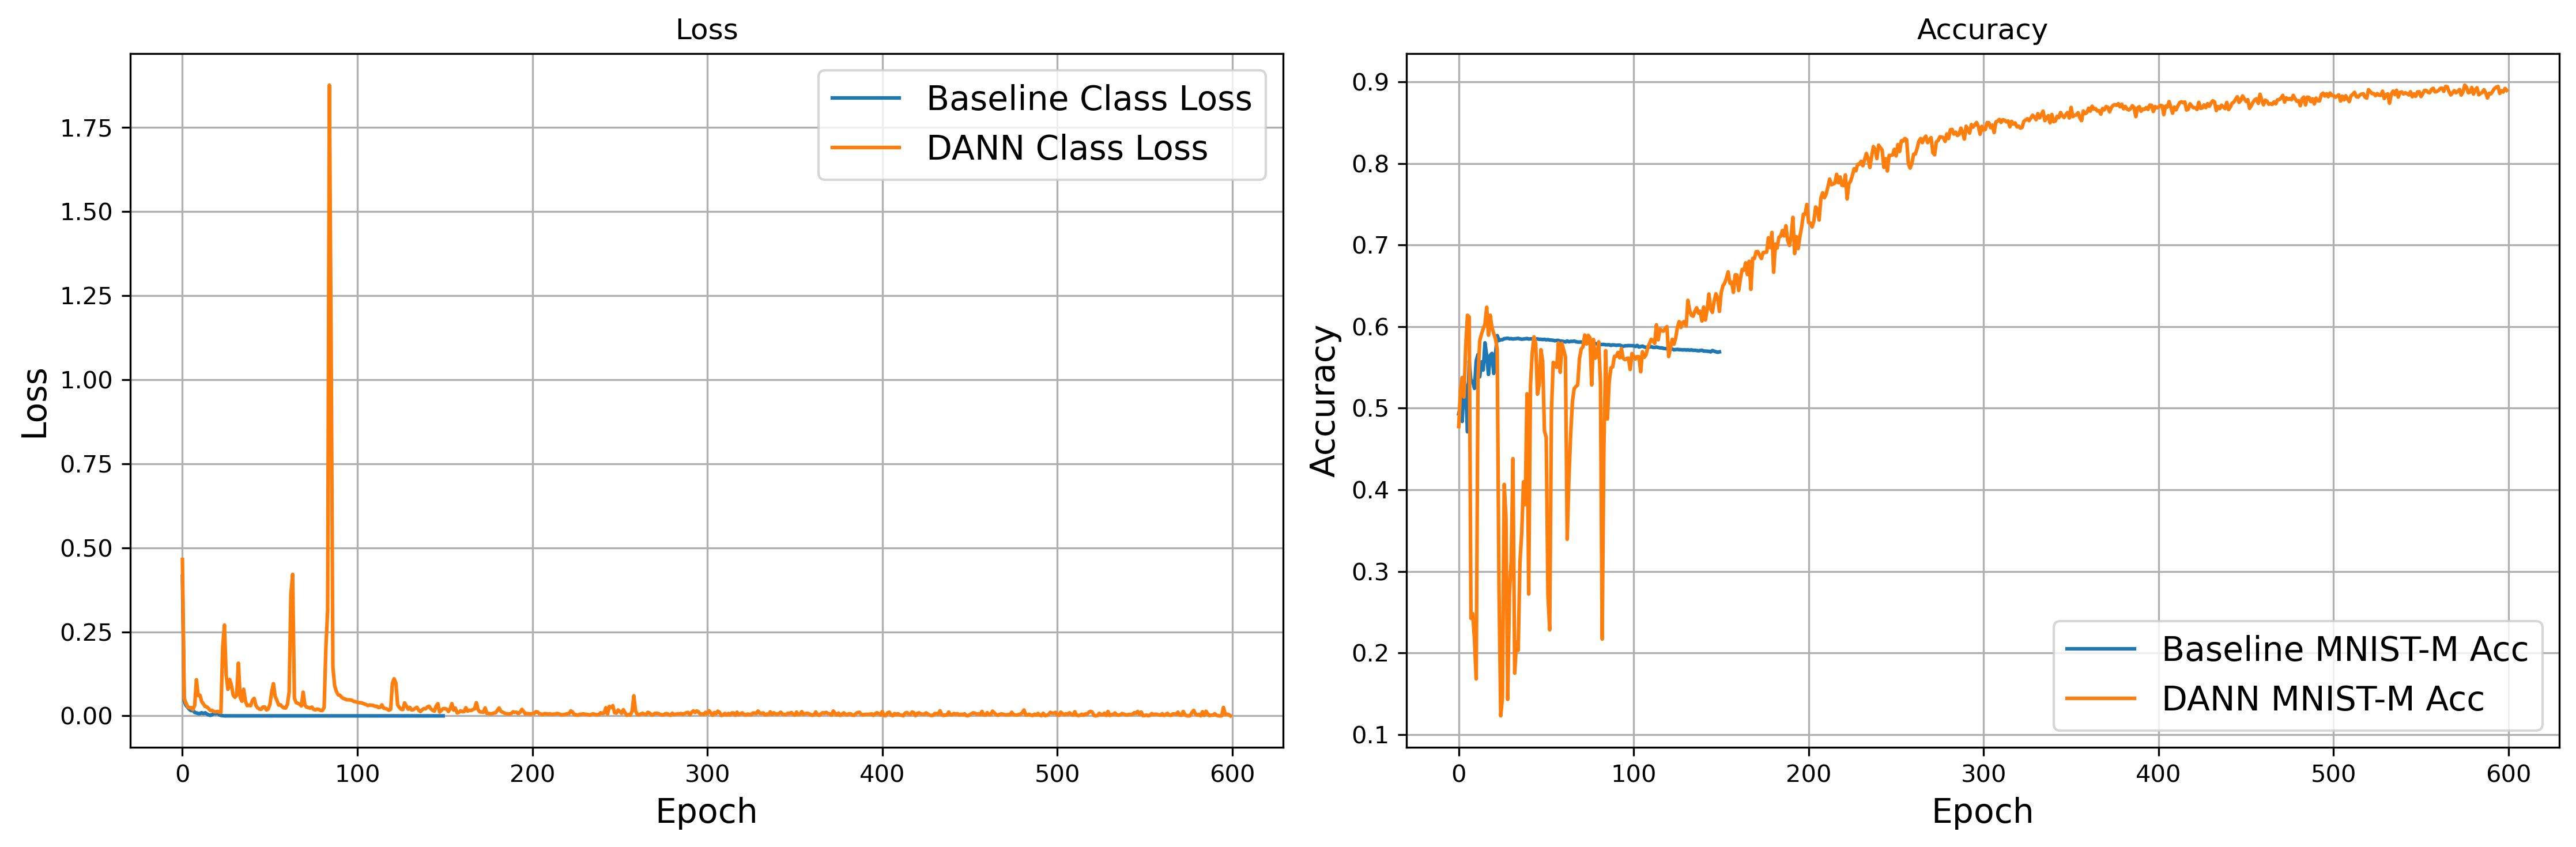
\includegraphics[width=0.8\textwidth]{../images/dann/dann_baseline_training.png}
    \caption{Perdida de clasificación y accuracy durante el entrenamiento del baseline y DANN.}
    \label{fig:dann baseline training}
\end{figure}

En la figura~\ref{fig:dann baseline training} para la loss de clasificación se observa que el baseline converge rápidamente, aproximadamente en la época 25. Sin embargo, a partir de ese punto su accuracy sobre MNIST-M empieza a disminuir levemente, lo que puede significar un sobre ajuste sobre MNIST y una perdida de generalización entre dominios. 

En cambio, DANN presenta un entrenamiento más ruidoso, con picos en la pérdida posiblemente asociados a la dinámica adversarial introducida por el discriminador de dominio y la GRL. A pesar de esa inestabilidad inicial, el modelo logra reducir progresivamente la pérdida y aumentar de manera sostenida la accuracy sobre MNIST-M, alcanzando un desempeño superior al baseline. Esto indica que el entrenamiento adversarial favorece la construcción de representaciones más transferibles entre dominios.

\begin{table}[h!]
\centering

\begin{tabular}{|l|c|c|c|}
\hline
 & MNIST (\%) & MNIST-M (\%)\\
\hline
Baseline & 99.51 & 56.45\\
\hline
DANN & 99.06 & 86.35\\
\hline
\end{tabular}
\caption{Accuracies sobre test de los modelos baseline y DANN para los tres dominios.}
\label{tab:tabla dann}
\end{table}

A partir de la tabla~\ref{tab:tabla dann}, se observa que el baseline obtiene un rendimiento apenas superior en MNIST, con una diferencia de $0.45\%$ respecto de DANN. Sin embargo, en MNIST-M la diferencia se invierte de manera significativa: DANN alcanza una accuracy de $86.35\%$, frente al $56.45\%$ del baseline, una mejora de aproximadamente $30\%$ en el dominio objetivo. Este resultado tiene sentido al considerar que baseline se entrena solamente para clasificar MNIST, mientras que DANN usa parte de su optimización para confundir al discriminador, logrando generalizar a MNIST-M.

\begin{figure}[H]
    \centering
    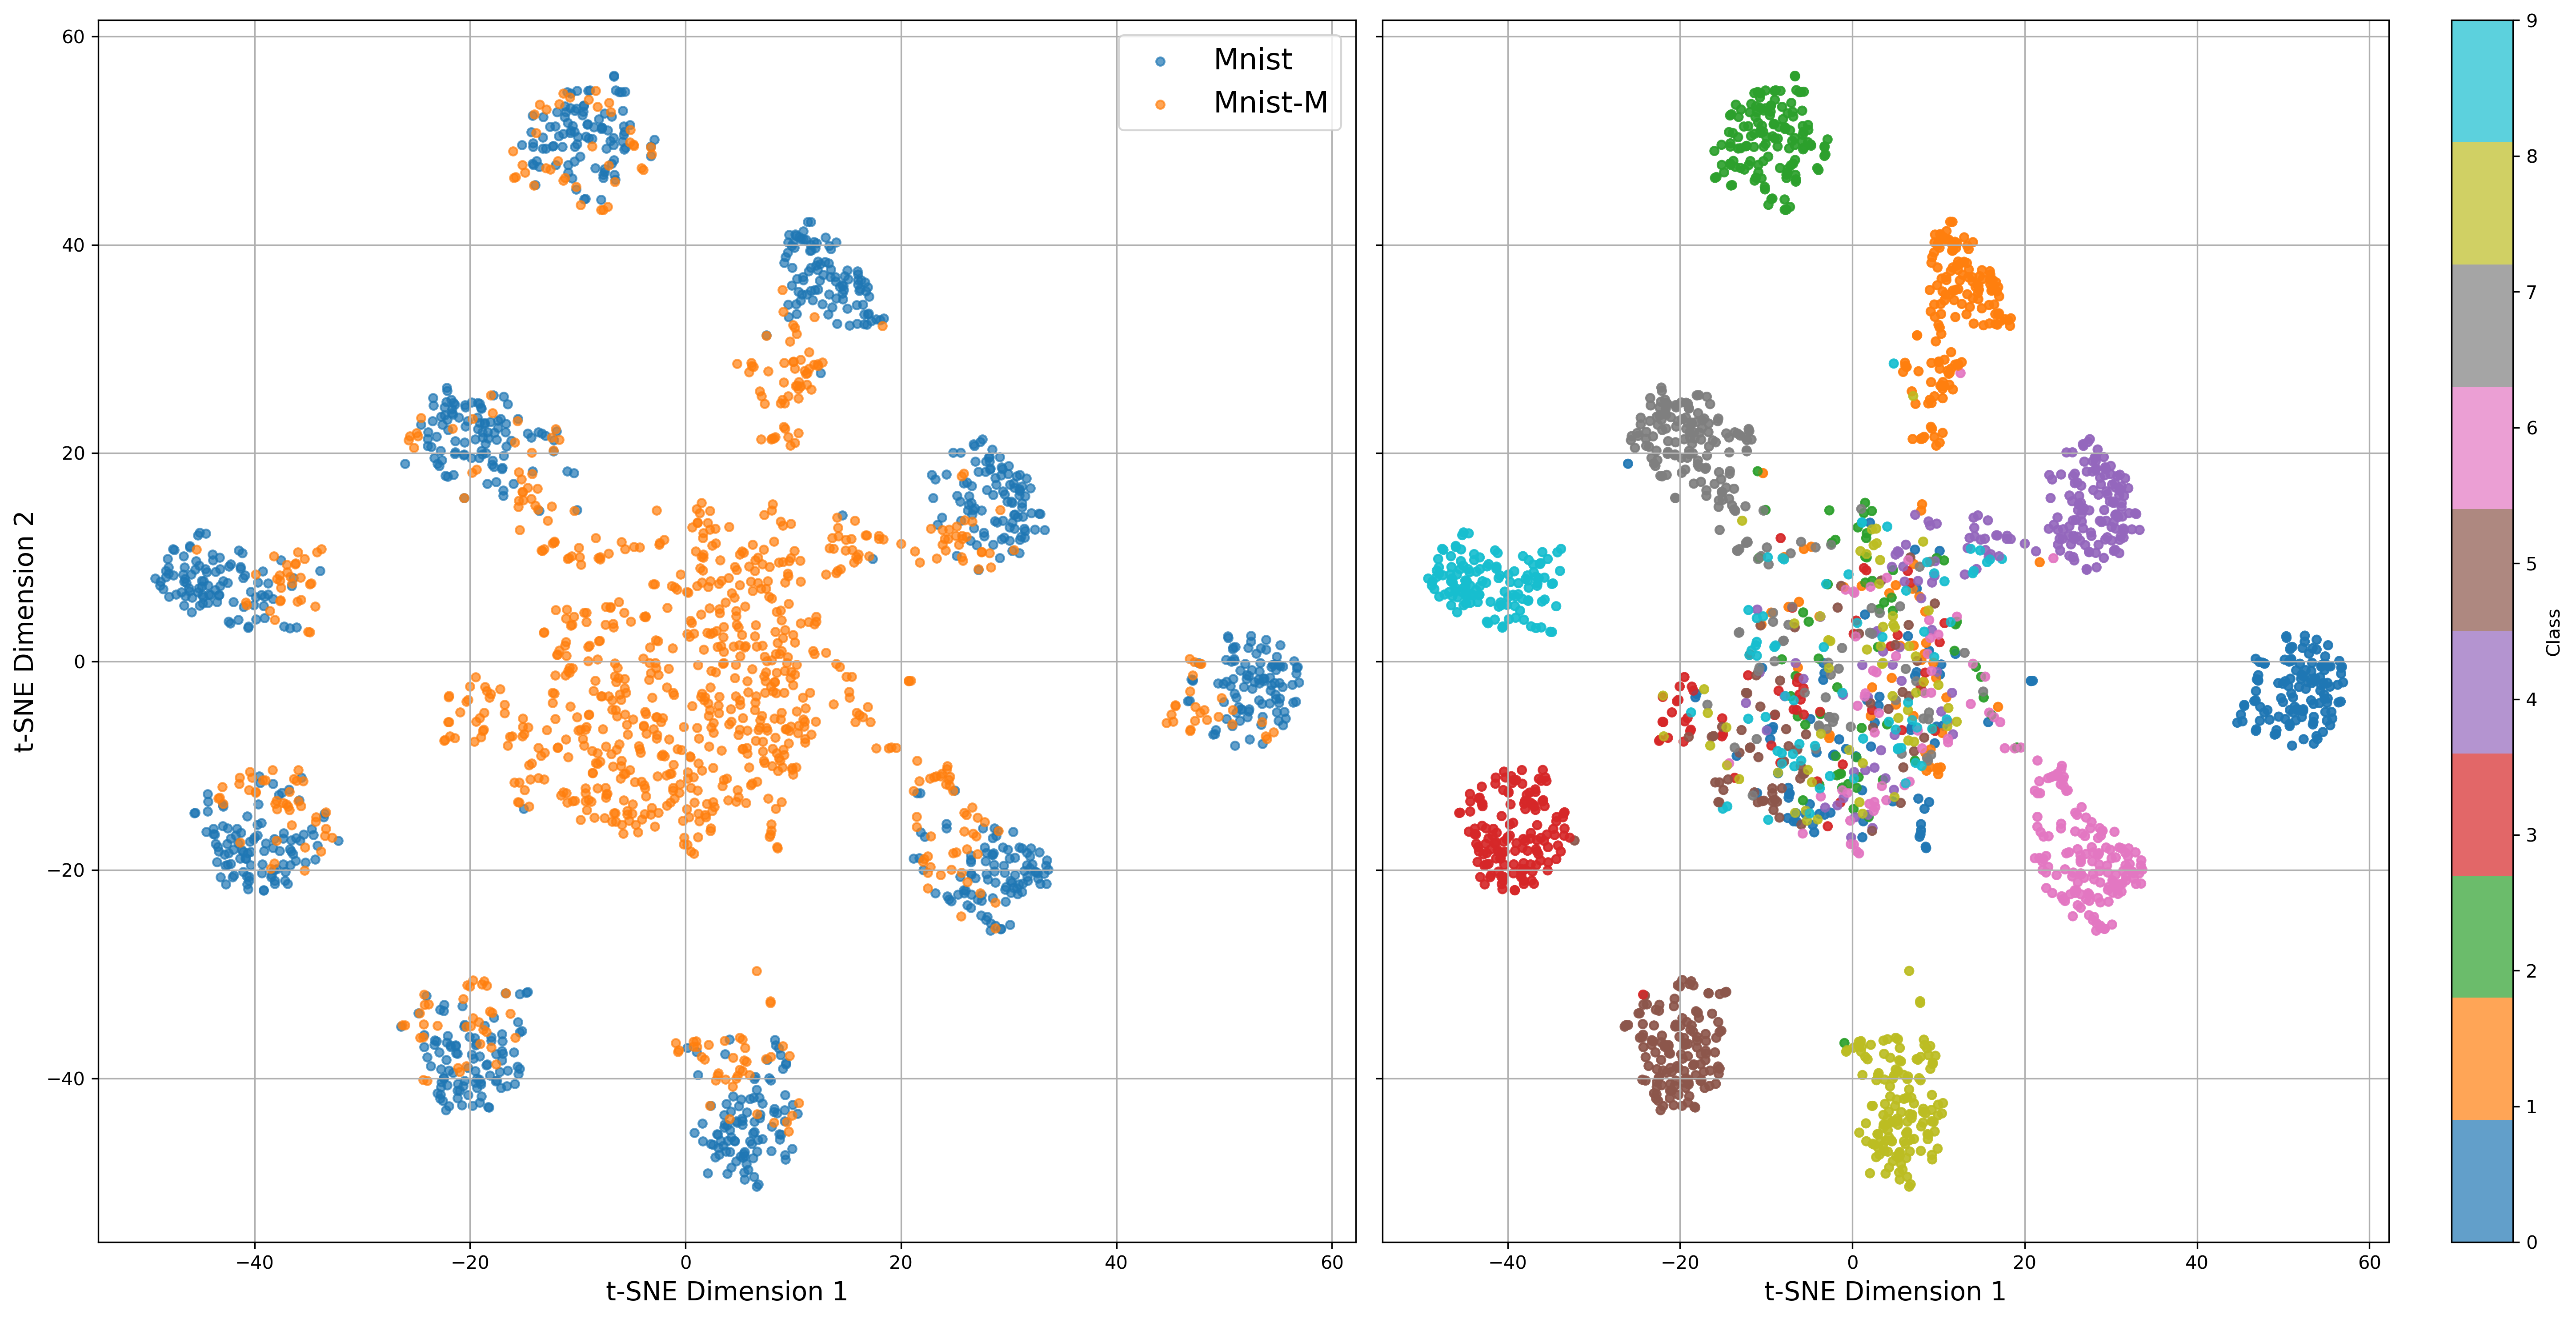
\includegraphics[width=0.8\textwidth]{../images/dann/baseline_tsne.png}
    \caption{t-SNE de los embeddings del encoder del baseline para un conjunto de imágene de prueba sobre MNIST y MNIST-M.}
    \label{fig:baseline tsne}
\end{figure}


\begin{figure}[H]
    \centering
    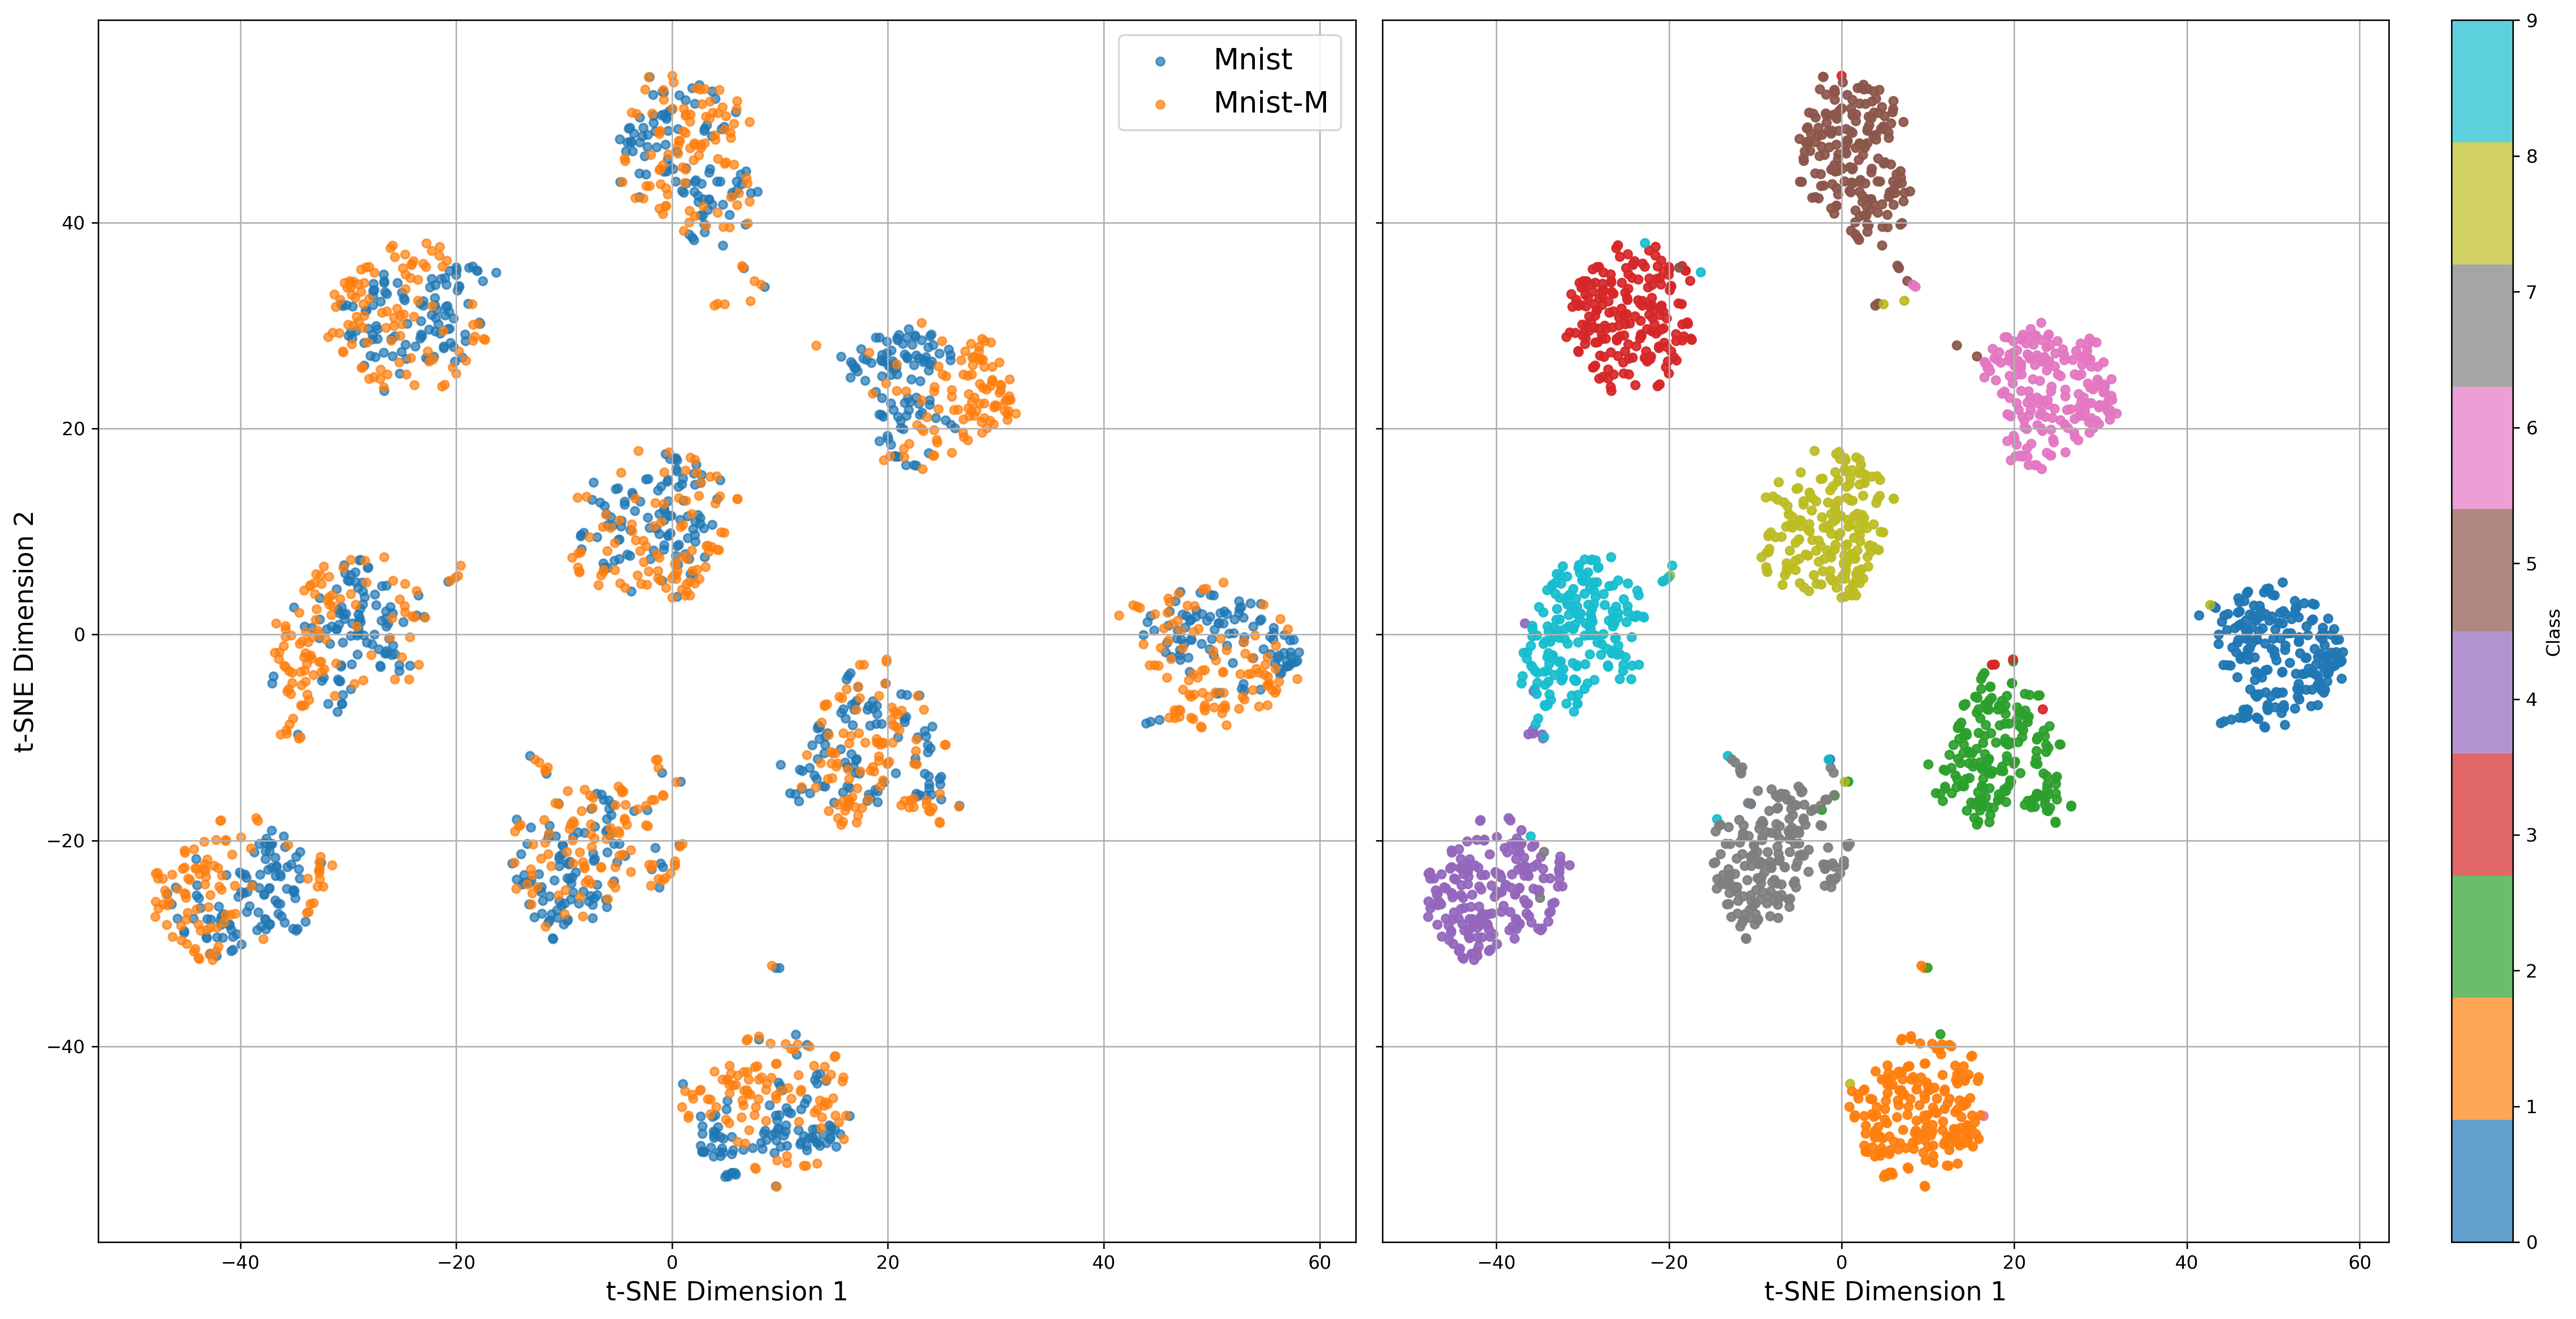
\includegraphics[width=0.8\textwidth]{../images/dann/baseline_ft_tsne.png}
    \caption{t-SNE de los embeddings del encoder del baseline finetuned para un conjunto de imágene de prueba sobre MNIST y MNIST-M.}
    \label{fig:baseline ft tsne}
\end{figure}


\begin{figure}[H]
    \centering
    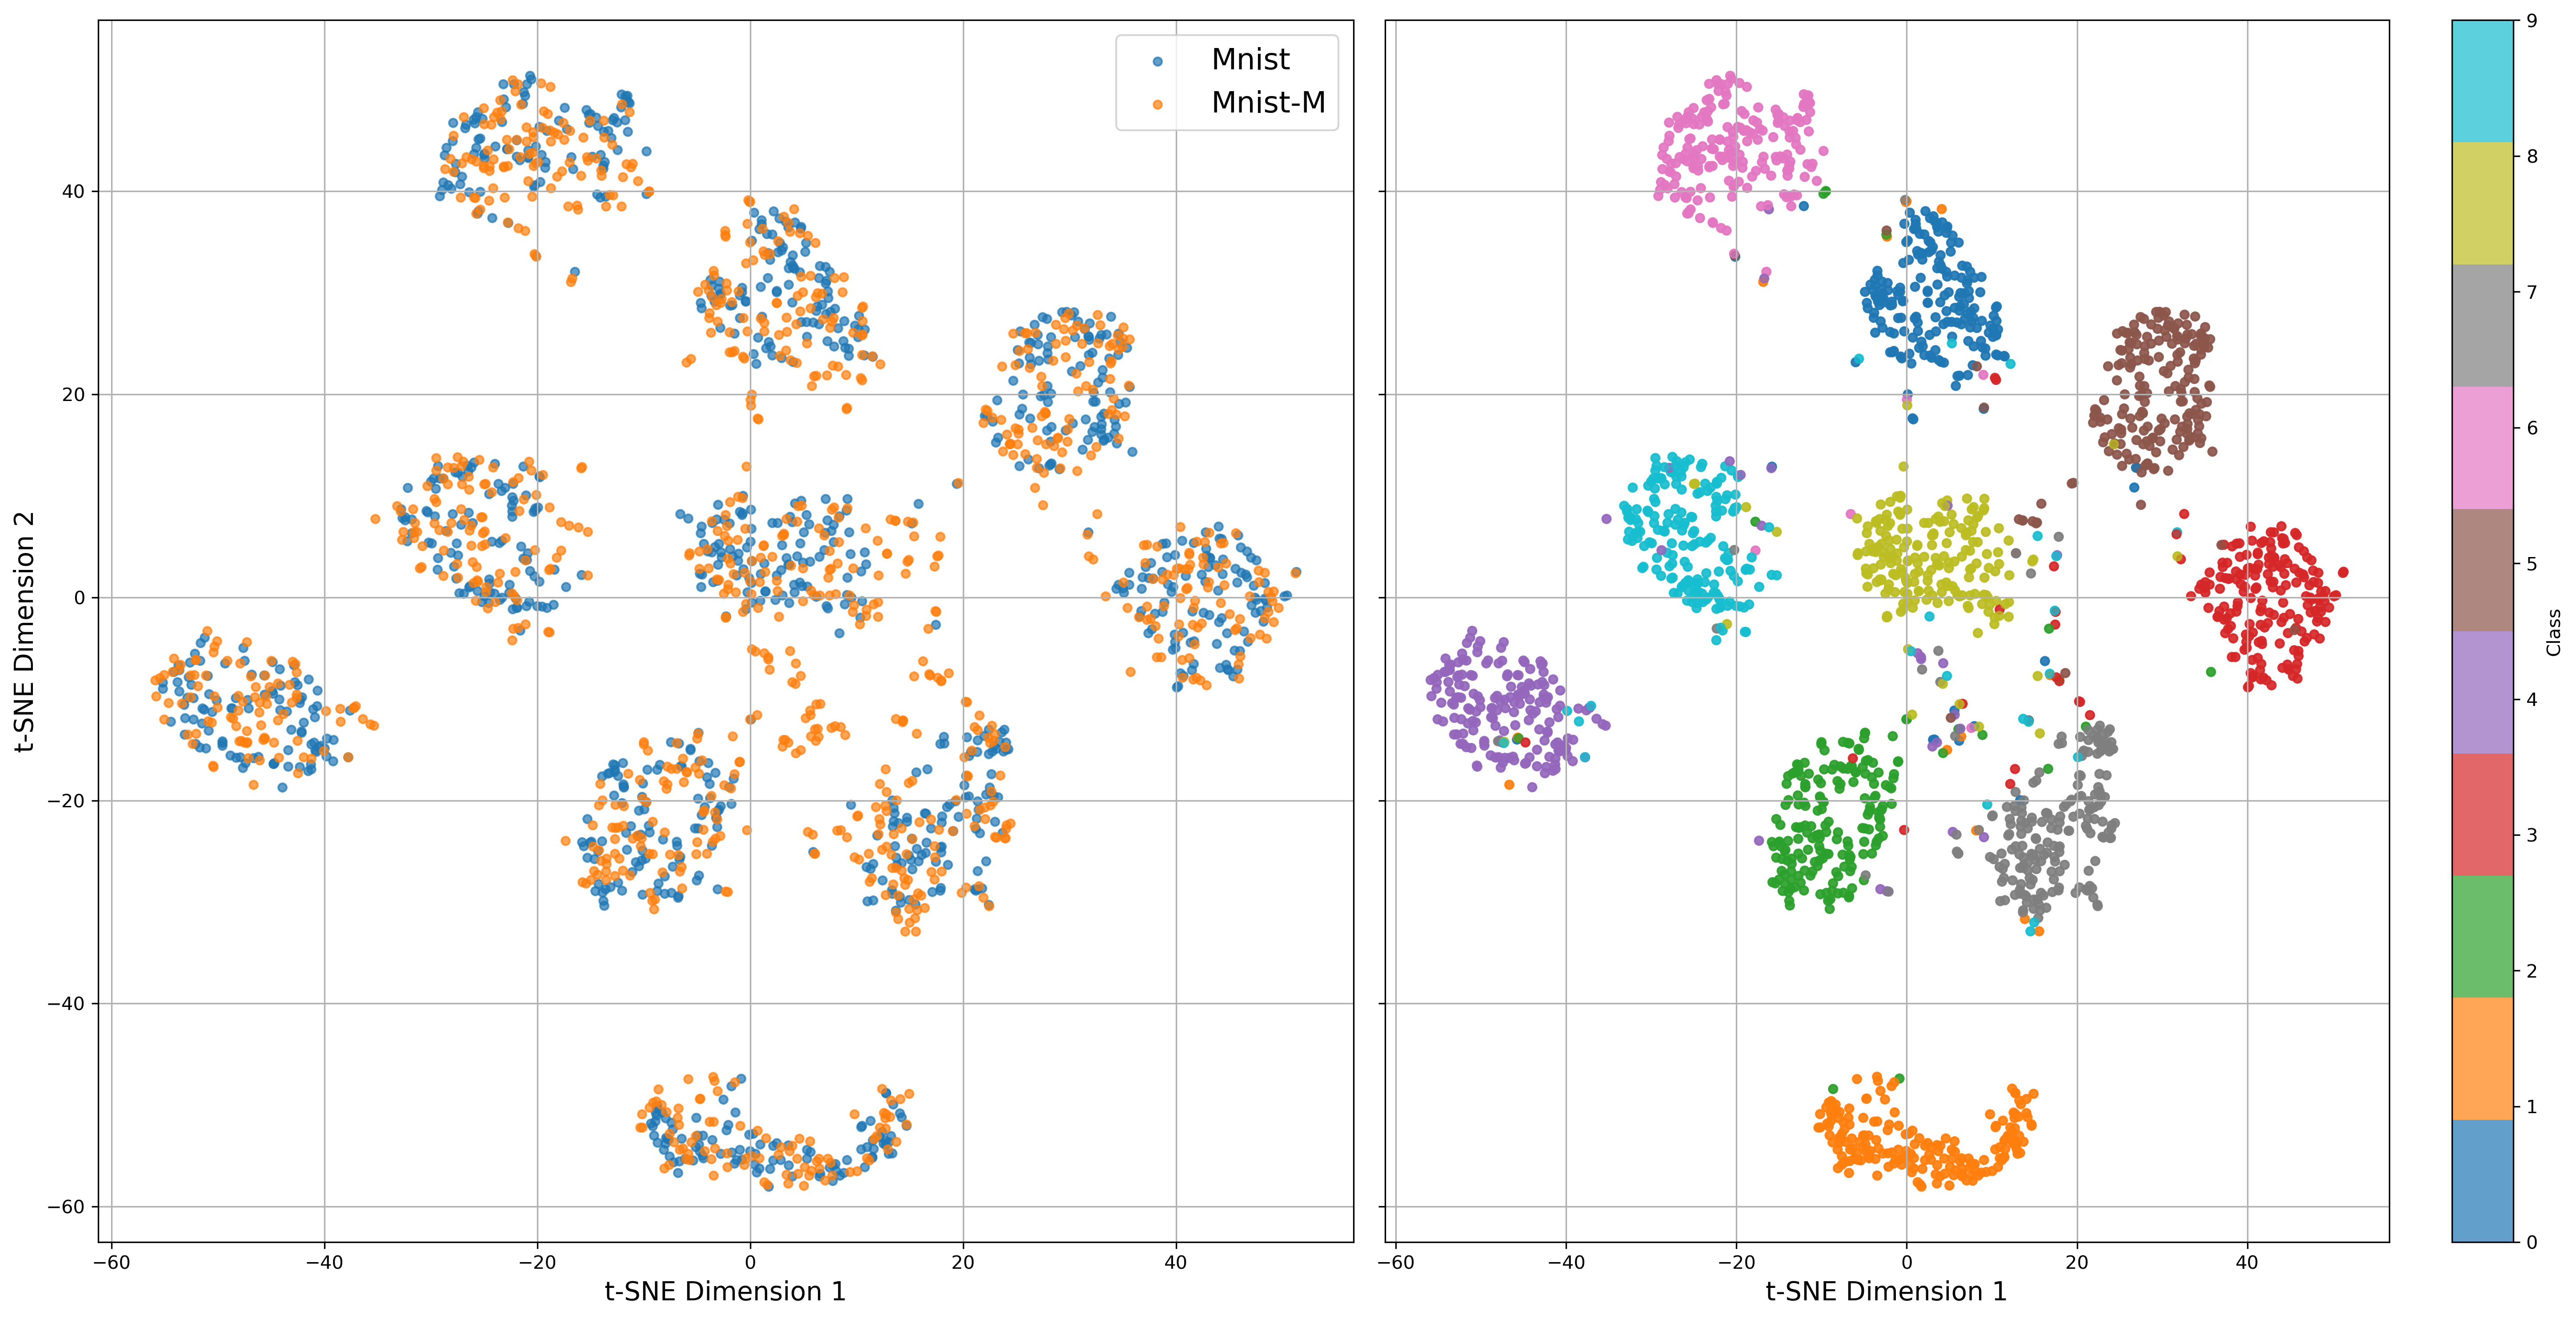
\includegraphics[width=0.8\textwidth]{../images/dann/dann_tsne.png}
    \caption{t-SNE de los embeddings del encoder de DANN para un conjunto de imágene de prueba sobre MNIST y MNIST-M.}
    \label{fig:dann tsne}
\end{figure}

A partir de las figuras~\ref{fig:baseline tsne},~\ref{fig:baseline ft tsne} y~\ref{fig:dann tsne}, se observa que el baseline es el modelo que presenta la peor organización del espacio latente. Si bien algunas clases de MNIST aparecen agrupadas, las muestras de MNIST-M quedan más dispersas y se concentran en una zona central con mayor mezcla entre clases.

Luego del fine-tuning, la separación por clase mejora de manera considerable: los clusters se vuelven más definidos y disminuye la mezcla entre muestras de distintas clases. Este resultado es esperable, ya que este modelo es el \textit{upper bound}.

Por su parte, DANN también muestra una mejora clara respecto del baseline. Los embeddings de MNIST y MNIST-M aparecen más alineados dentro de varios clusters, lo que sugiere que el entrenamiento adversarial favorece representaciones más invariantes al dominio. Aunque el baseline con fine-tuning logra una separación visual más limpia, DANN obtiene esta mejora mediante adaptación adversarial, sin depender de un ajuste supervisado sobre el dominio objetivo.  

\section{Conclusión}
En este trabajo se estudiaron distintos métodos de meta-learning y domain adaptation aplicados a tareas de clasificación de dígitos bajo escenarios de cambio de dominio con pocos ejemplos.

En primer lugar, la evaluación de ProtoNet, MAML y ProtoMAML sobre MNIST-M y SVHN permitió observar con claridad el impacto del cambio de dominio. Aunque MNIST-M mantiene cierta similitud estructural con MNIST, sobre este dominio se reduce el desempeño. En SVHN, esta caída es aún más marcada, ya que las imágenes provienen de un contexto con mayor variabilidad de distintos aspectos. 

Entre los métodos de meta-learning comparados, ProtoNet y ProtoMAML obtuvieron mejores resultados que MAML en los dominios externos. Este comportamiento sugiere que los enfoques basados en representaciones prototípicas son más robustos frente al cambio de dominio que una adaptación basada únicamente en gradientes con muy pocos ejemplos. Además, ProtoMAML logró resultados similares o superiores a ProtoNet aun habiendo sido entrenado en la mitad de iteraciones y con menor cantidad de ejemplos por clase, lo que indica que la combinación entre inicialización prototípica y adaptación interna puede ser una estrategia efectiva para escenarios few-shot.

Por otro lado, los experimentos de domain adaptation mostraron que DANN mejora de manera significativa la transferencia de MNIST a MNIST-M respecto del baseline. Mientras que el baseline alcanza una accuracy alta sobre MNIST pero cae considerablemente en MNIST-M, DANN mantiene un rendimiento similar en el dominio fuente y obtiene una mejora importante en el dominio objetivo ($30\%$). Este resultado confirma que el entrenamiento adversarial mediante la Gradient Reversal Layer favorece la construcción de embeddings más invariantes al dominio, permitiendo que el modelo aproveche información no etiquetada del dominio target sin necesidad de realizar un ajuste supervisado completo.

El análisis de los embeddings mediante t-SNE acompaña esta interpretación: los modelos entrenados únicamente sobre MNIST tienden a organizar mejor las muestras del dominio fuente, pero presentan mayor dispersión y mezcla cuando se incorporan muestras de MNIST-M o SVHN. En cambio, DANN logra una mejor alineación entre MNIST y MNIST-M, lo que explica su mejora en accuracy sobre el dominio objetivo. De todas formas, el baseline con fine-tuning obtiene la separación más clara, algo esperable porque utiliza etiquetas del dominio target y funciona como una cota superior supervisada.

Como trabajo futuro, sería interesante incorporar técnicas de data augmentation para aumentar la variabilidad visual durante el entrenamiento y mejorar la robustez de los embeddings frente a cambios de dominio. También podrían evaluarse estrategias de adaptación más avanzadas, diferentes arquitecturas de encoder o combinaciones entre meta-learning y domain adaptation, con el objetivo de obtener modelos que no solo aprendan con pocos ejemplos, sino que además puedan generalizar mejor a dominios visualmente distintos.
% \end{multicols}

\newpage
\section{Bibliografía}
1. Snell, J., Swersky, K. \& Zemel, R. S. (2017). Prototypical Networks for Few-shot Learning. Advances in Neural Information Processing Systems, 30. Disponible en: \url{https://arxiv.org/abs/1703.05175}

2. Finn, C., Abbeel, P. \& Levine, S. (2017). Model-Agnostic Meta-Learning for Fast Adaptation of Deep Networks. Proceedings of the 34th International Conference on Machine Learning, PMLR 70, 1126--1135. Disponible en: \url{https://arxiv.org/abs/1703.03400}

3. Triantafillou, E., Zhu, T., Dumoulin, V., Lamblin, P., Evci, U., Xu, K., Goroshin, R., Gelada, C., Swersky, K., Manzagol, P.-A. \& Larochelle, H. (2020). Meta-Dataset: A Dataset of Datasets for Learning to Learn from Few Examples. International Conference on Learning Representations. Disponible en: \url{https://arxiv.org/abs/1903.03096}

4. Ganin, Y., Ustinova, E., Ajakan, H., Germain, P., Larochelle, H., Laviolette, F., Marchand, M. \& Lempitsky, V. (2016). Domain-Adversarial Training of Neural Networks. Journal of Machine Learning Research, 17(59), 1--35. Disponible en: \url{https://arxiv.org/abs/1505.07818}


\end{document}
